% CVPR 2024 Paper Template; see https://github.com/cvpr-org/author-kit

\documentclass[10pt,twocolumn,letterpaper]{article}

%%%%%%%%% PAPER TYPE  - PLEASE UPDATE FOR FINAL VERSION
% \usepackage[review]{cvpr}      % To produce the REVIEW version
% \usepackage{cvpr}              % To produce the CAMERA-READY version
\usepackage[pagenumbers]{cvpr} % To force page numbers, e.g. for an arXiv version

% Include other packages here, before hyperref.
\usepackage{graphicx}
\usepackage{amsmath}
\usepackage{amssymb}
\usepackage{booktabs}
\usepackage{algpseudocode}
\usepackage{algorithm}
\usepackage{mathtools}
\usepackage{stmaryrd}
\usepackage{trimclip}
\newcommand{\X}{\mathbf{X}} %
\newcommand{\Xset}{{\cal X}} %
\newcommand{\T}{\mathbf{T}} %
\newcommand{\Tset}{\mathcal{T}} %
\newcommand{\Tp}{\tilde{\mathbf{T}}} %
\newcommand{\Rp}{\tilde{\mathbf{R}}} %
\newcommand{\tp}{\tilde{\mathbf{t}}} %
\newcommand{\G}{\mathbf{G}} %
\newcommand{\Edge}{\mathcal{E}} %
\newcommand{\Gset}{\mathcal{G}} %
\newcommand{\g}{\mathbf{g}} %
\newcommand{\flow}{\mathbf{F}} %
\newcommand{\fpt}{\bm{f}} %
\newcommand{\Pm}{\mathbf{P}} %
\newcommand{\Pset}{\mathcal{P}} %
\newcommand{\Id}{\mathbf{I}} %
\newcommand{\R}{\mathbb{R}} %
\newcommand{\Rot}{\mathbf{R}} %
\newcommand{\tra}{\mathbf{t}} %
\newcommand{\Lap}{\mathbf{L}} %
\newcommand{\w}{\mathbf{w}} %
\newcommand{\Z}{\bm{\zeta}} %
\newcommand{\Zm}{\mathbf{Z}} %
\newcommand{\U}{\mathbf{U}} %
\newcommand{\segnet}{\varphi_{\mathrm{group}}} %
\newcommand{\flownet}{\varphi_{\mathrm{flow}}} %
\newcommand{\confnet}{\varphi_{\mathrm{conf}}} %
\newcommand{\Man}{\mathcal{M}} %
\newcommand{\one}{\mathbf{1}} %
\newcommand{\zero}{\mathbf{0}} %
\newcommand{\SOg}{\mathrm{SO}(3)} %
\newcommand{\Sm}{\mathbf{S}} %
\newcommand{\D}{\mathbf{D}} %
\newcommand{\gt}{\mathrm{gt}}   %
\newcommand{\wt}{\mathbf{w}}    %
\newcommand{\cf}{\textit{cf.}}    %
\newcommand{\wrt}{\text{w.r.t.}}
\newcommand{\etal}{\textit{et al.}}
\newcommand{\refpaper}[1]{{\hypersetup{linkcolor={blue}}\ref{#1}}}

\newcommand{\mydots}{...}


\newcolumntype{Y}{>{\centering\arraybackslash}X}

\newtheorem{thm}{Theorem}
\newtheorem{remark}{Remark}
\newtheorem{cor}{Corollary}
\newtheorem{lemma}{Lemma}
\newtheorem{prop}{Proposition}
\newtheorem{dfn}{Definition}
\newtheorem{conj}{Conjecture}


\newcommand{\tmpeqno}{{\color{red} (TEMPEQ) }}

\newcommand{\jh}[1]{\textcolor[rgb]{0.0,0.0,1.0}{(Jiahui: #1)}}
\newcommand{\tolga}[1]{{\color{red} (Tolga: #1)} }

% \DeclareMathOperator{\sign}{sign}
\newcommand{\sign}{\operatorname{sign}}
\newcommand{\sas}{{\cal S} \alpha {\cal S} }

\crefname{section}{\S}{\S\S}
\crefname{subsection}{\S}{\S\S}

\newtheorem{assumption}{\textbf{H}\hspace{-3pt}}
\Crefname{assumption}{\textbf{H}\hspace{-3pt}}{\textbf{H}\hspace{-3pt}}
\crefname{assumption}{\textbf{H}}{\textbf{H}}

\newcommand{\insertimage}[4]{ %
\begin{figure}[t]
\centering
\includegraphics[scale=#1, clip=true]{figures/#2}
\caption{#3}
\label{#4}
\end{figure}
}

\newcommand{\insertimageC}[5]{ %
\begin{figure}[#5]
\centering
\includegraphics[width=#1\columnwidth, clip=true]{figures/#2}
\caption{#3}
\label{#4}
\end{figure}
}


\newcommand{\insertimageStar}[5]{ %
\begin{figure}[#5]
\centering
\includegraphics[width=#1\columnwidth, clip=true]{figures/#2}
\caption{#3}
\label{#4}
\end{figure}
}

\newcommand{\insertimageAsSubfig}[5]{ %
\begin{figure}[#5]
\begin{center}
\subfigbottomskip =-4in
\subfigure{
\includegraphics[width=#1\columnwidth]{figures/#2}
\label{#4}
}
\end{center}
\subfigbottomskip =-4in
\caption{#3}
\label{#4}
\end{figure}
}

\newcolumntype{d}[1]{D{.}{.}{#1}}
\newcolumntype{B}[3]{>{\boldmath\DC@{#1}{#2}{#3}}c<{\DC@end}}
% \DeclareMathOperator*{\argmax}{argmax}
\newcommand{\argmax}{\operatorname{argmax}}
% \DeclareMathOperator*{\argmin}{argmin}
\newcommand{\argmin}{\operatorname{argmin}}
\definecolor{tikz_gray}{RGB}{191,191,191}
\definecolor{tikz_lblue}{RGB}{93,138,210}
\definecolor{tikz_dblue}{RGB}{46,78,124}
\definecolor{tikz_lviolet}{RGB}{161,125,173}
\definecolor{tikz_dviolet}{RGB}{148,55,255}
\definecolor{tikz_rose}{RGB}{250,150,150}
\definecolor{tikz_pink}{RGB}{214,19,115}
\definecolor{tikz_lpink}{RGB}{255,138,216}

\newcommand{\overbar}[1]{\mkern 1.5mu\overline{\mkern-1.5mu#1\mkern-1.5mu}\mkern 1.5mu}

\DeclareRobustCommand{\legendsquare}[1]{%
  \tikz[baseline=(a.south)]{\node[#1, inner sep=.8ex, outer sep=0] (a) {};}%
}
\newcommand{\parahead}[1]{\noindent\textbf{#1}:\ }
\newcommand{\tabhead}[1]{\par\textbf{#1}}
\newenvironment{packed_itemize}
{\begin{itemize}
    \setlength{\itemsep}{1pt}
    \setlength{\parskip}{0pt}
    \setlength{\parsep}{0pt}
}{\end{itemize}}


\newcommand{\konrad}[1]{{\textcolor{blue}{\textbf{Konrad:} {#1}}}}
\newcommand{\andreas}[1]{{\textcolor{cyan}{\textbf{Andreas:} {#1}}}}
\newcommand{\zan}[1]{{\textcolor{brown}{\textbf{Zan:} {#1}}}}
\newcommand{\shengyu}[1]{{\textcolor{magenta}{\textbf{Shengyu:} {#1}}}}
\newcommand{\mikhail}[1]{{\textcolor{orange}{\textbf{Mikhail:} {#1}}}}
\newcommand{\cameraready}[1]{{\textcolor{blue}{{#1}}}}

\newcommand{\acro}{\textsc{Predator}}
\newcommand{\acroexplain}{\textbf{p}oint-cloud \textbf{re}gistration with \textbf{d}eep \textbf{at}tention to the \textbf{o}verlap \textbf{r}egion}





\sloppy
\definecolor{turquoise}{cmyk}{0.65,0,0.1,0.3}
\definecolor{purple}{rgb}{0.65,0,0.65}
\definecolor{dark_green}{rgb}{0, 0.5, 0}
\definecolor{orange}{rgb}{0.8, 0.6, 0.2}
\definecolor{red}{rgb}{0.8, 0.2, 0.2}
\definecolor{darkred}{rgb}{0.6, 0.1, 0.05}
\definecolor{blueish}{rgb}{0.0, 0.3, .6}
\definecolor{light_gray}{rgb}{0.7, 0.7, .7}
\definecolor{pink}{rgb}{1, 0, 1}
\definecolor{greyblue}{rgb}{0.25, 0.25, 1}


\newcommand{\CIRCLE}[1]{\raisebox{.5pt}{\footnotesize \textcircled{\raisebox{-.6pt}{#1}}}}

\newcommand{\expect}{\mathbb{E}}
\newcommand{\real}{\mathbb{R}}
\newcommand{\waymo}{\emph{Waymo}}
\newcommand{\nuscenes}{\emph{nuScenes}}

\crefname{section}{\S}{\S\S}
\crefname{subsection}{\S}{\S\S}
\crefname{equation}{\text{Eq}}{\text{Eq}}
\crefname{definition}{\text{Dfn.}}{\text{Dfn.}}
\crefname{tab}{\text{Tab.}}{\text{Tab.}}
\crefname{fig}{\text{Fig.}}{\text{Fig.}}
\crefname{table}{\text{Tab.}}{\text{Tab.}}
\crefname{figure}{\text{Fig.}}{\text{Fig.}}

\usepackage{blindtext}
\newcommand{\lorem}[1]{\todo{\blindtext[#1]}}

\renewcommand{\paragraph}[1]{\vspace{1em}\noindent\textbf{#1}.}


\newcommand{\lcircle}[1]{{\hspace{0.1em}\tikz\draw[#1,fill=#1] (0,0) circle (.4ex);}}

\makeatletter
\DeclareRobustCommand\onedot{\futurelet\@let@token\@onedot}
\def\@onedot{\ifx\@let@token.\else.\null\fi\xspace}

\def\eg{\emph{e.g}\onedot} \def\Eg{\emph{E.g}\onedot}
\def\ie{\emph{i.e}\onedot} \def\Ie{\emph{I.e}\onedot}
\def\cf{\emph{c.f}\onedot} \def\Cf{\emph{C.f}\onedot}
\def\etc{\emph{etc}\onedot} \def\vs{\emph{vs}\onedot}
\def\wrt{w.r.t\onedot} \def\dof{d.o.f\onedot}
\def\etal{\emph{et al}\onedot}
\makeatother

\newcommand{\ego}{\mathrm{ego}}
\newcommand{\pos}{\mathrm{pos}}
\newcommand{\geo}{\mathrm{ego}}     %
\newcommand{\pose}{\mathrm{pose}}
\newcommand{\obj}{\mathrm{obj}}
\newcommand{\trans}{\mathrm{trans}}
\newcommand{\type}{*}
\newcommand{\static}{\mathrm{static}}
\newcommand{\loss}{\mathcal{L}}
\newcommand{\Iset}{\mathcal{I}}
\newcommand{\tvec}{\mathbf{t}}
\newcommand{\Flow}{\mathbf{V}}
\newcommand{\s}{\mathbf{s}}
\newcommand{\x}{\mathbf{x}}
\newcommand{\quat}{\mathbf{q}}
\newcommand{\SEuc}{\mathrm{SE}(3)}
\newcommand{\Feature}{\mathbf{F}}
\newcommand{\feature}{\mathbf{f}}
\newcommand{\agfeature}{\tilde{\mathbf{f}}}
\newcommand{\pillar}{\mathbf{p}}
\newcommand{\point}{\mathbf{x}}
\newcommand{\offset}{\bm{\delta}}
\newcommand{\MLP}{\mathrm{MLP}}
\newcommand{\PN}{\mathrm{PN}}
\newcommand{\FG}{\mathrm{FG}}
\newcommand{\cat}{\mathrm{cat}}
\newcommand{\textoffset}{\mathrm{offset}}
\newcommand{\PC}{\mathbf{X}}
\newcommand{\PCset}{\mathcal{X}}
\newcommand{\bev}{\mathrm{base}}  %
\newcommand{\motion}{\mathrm{motion}}  %

\definecolor{lossred}{rgb}{1.0, 0.01, 0.24}
\definecolor{lossgreen}{rgb}{0.55, 0.71, 0.0}
\definecolor{lossblue}{rgb}{0.0, 0.44, 1.0}
\definecolor{lossyellow}{rgb}{1.0, 0.66, 0.07}
\definecolor{losspurple}{rgb}{0.76, 0.33, 0.76}
\definecolor{tab10orange}{rgb}{1.0, 0.7, 0.0}




\newcommand{\todo}[1]{{\textcolor{red}{\textbf{#1}}}}

\newcommand{\btau}{\boldsymbol{\tau}}
\newcommand{\bmu}{\boldsymbol{\mu}}
\newcommand{\beps}{\boldsymbol{\epsilon}}
\newcommand{\ba}{\mathbf{a}}
\newcommand{\bx}{\mathbf{x}}
\newcommand{\bc}{\mathbf{c}}

\newcommand{\map}{\boldsymbol{\mathcal{M}}}
\newcommand{\reals}{\mathbb{R}}
\newcommand{\normal}{\mathcal{N}}
\newcommand{\guide}{\mathcal{J}}


\newcommand{\name}{{{NeLF}}\xspace}

\definecolor{mygray}{RGB}{120, 120, 120}
\definecolor{myblue}{RGB}{68, 114, 196}
\definecolor{myorange}{RGB}{237, 125, 49}

\newcommand{\dir}{\mathbf{d}}
\newcommand{\origin}{\mathbf{o}}
\newcommand{\f}{\mathbf{f}}
\newcommand{\ray}{\mathbf{r}}
\newcommand{\density}{\sigma}
\newcommand{\opacity}{\alpha}
\newcommand{\reflectance}{\rho}
\newcommand{\radiance}{\mathbf{c}}
\newcommand{\intensity}{e}
\newcommand{\pdrop}{p_d}
\newcommand{\ptwo}{p_s}
\newcommand{\posfeat}{\mathbf{f}_{\text{pos}}}
\newcommand{\geofeat}{\mathbf{f}_{\text{geo}}}
\newcommand{\geofeatbar}{\bar{\mathbf{f}}_{\text{geo}}}
\newcommand{\dirfeat}{\mathbf{f}_{\text{dir}}}
\newcommand{\rangefeat}{\mathbf{f}_{\text{range}}}
\newcommand{\rayfeat}{\mathbf{f}_{\text{beam}}}
\definecolor{sem0}{rgb}{0.98431373, 0.70588235, 0.68235294}
\definecolor{sem1}{rgb}{0.70196078,0.80392157, 0.89019608}
\definecolor{sem2}{rgb}{0.8, 0.92156863, 0.77254902}
\definecolor{sem3}{rgb}{0.87058824, 0.79607843, 0.89411765}
\definecolor{ourgray}{rgb}{0.78, 0.78, 0.78}
\definecolor{error}{rgb}{0, 0.635, 1}
\definecolor{sdpoints}{rgb}{1.0, 0.706, 0.0}
\definecolor{hit}{rgb}{0.12156863,0.47058824,0.70588235}
\newcommand{\coolwarm}{
\includegraphics[width=3em,height=0.8em]{content/main/images/coolwarm.png}}
\newcommand{\bwr}{
\includegraphics[width=3em,height=0.8em]{content/main/images/bwr.png}}



\DeclarePairedDelimiter\parens{\lparen}{\rparen}
\DeclarePairedDelimiter\abs{\lvert}{\rvert}
\DeclarePairedDelimiter\norm{\lVert}{\rVert}
\DeclarePairedDelimiter\floor{\lfloor}{\rfloor}
\DeclarePairedDelimiter\ceil{\lceil}{\rceil}
\DeclarePairedDelimiter\braces{\lbrace}{\rbrace}
\DeclarePairedDelimiter\bracks{\lbrack}{\rbrack}
\DeclarePairedDelimiter\angles{\langle}{\rangle}

\crefname{section}{Sec.}{Secs.}
\Crefname{section}{Section}{Sections}
\Crefname{table}{Table}{Tables}
\crefname{table}{Tab.}{Tabs.}
\crefname{equation}{\text{Eq}}{\text{Eq}}
\crefname{equation}{Eq.}{Eq.}

\makeatletter
 \def\@textbottom{\vskip \z@ \@plus 1pt}
 \let\@texttop\relax
\makeatother


\newcommand{\dynfl}{DyNFL\xspace}
\newcommand{\rgb}{\mathbf{c}}
\newcommand{\pt}{\mathbf{p}}
\newcommand{\feat}{\gamma}
\newcommand{\tnt}{Tanks and Temples\xspace}
\newcommand{\deriv}[2]{\frac{\partial #1}{\partial #2}}
\newcommand{\sdf}{f}
\newcommand{\curv}{\frac{1}{2} \nabla^2 \sdf(\pos)}
\newcommand{\dist}{\mathbf{d_{f}}}
\newcommand{\leik}{\mathcal{L}_{\text{eik}}}
\newcommand{\transmittance}{\mathcal{T}}
\newcommand{\bwrDyNFL}{
\includegraphics[width=3em,height=0.8em]{Figures/bwr.png}}
\newcommand{\exponential}[1]{\text{exp}\left(#1\right)}
\newcommand{\rayfeatideal}{\mathbf{f}_{\text{ray}}}
\newcommand{\reflectivity}{\rho}
\newcommand{\weight}{\alpha}
\newcommand{\rayOri}{\mathbf{o}}
\newcommand{\rayDir}{\mathbf{d}}

\makeatletter
\DeclareRobustCommand{\shortto}{%
  \mathrel{\mathpalette\short@to\relax}%
}

\newcommand{\short@to}[2]{%
  \mkern2mu
  \clipbox{{.5\width} 0 0 0}{$\m@th#1\vphantom{+}{\shortrightarrow}$}%
  }
\makeatother
\newcommand{\xing}[1]{{\textcolor{blue}{\textbf{Xing: {#1}}}}}
\newcommand{\shengyu}[1]{{\textcolor{red}{\textbf{Shengyu:} {#1}}}}
\newcommand{\orl}[1]{{\textcolor{orange}{\textbf{OrL:} {#1}}}}
\newcommand{\stefan}[1]{{\textcolor{pink}{\textbf{Stefan:} {#1}}}}
\newcommand{\hanfeng}[1]{{\textcolor{green}{\textbf{Hanfeng:} {#1}}}}
\newcommand{\dynfl}{DyNFL\xspace}
\newcommand{\dynfl}{DyNFL\xspace}
\allowdisplaybreaks
\newcommand{\rgb}{\mathbf{c}}
\newcommand{\pos}{\mathbf{p}}
\newcommand{\feat}{\gamma}
\newcommand{\tnt}{Tanks and Temples\xspace}
\newcommand{\deriv}[2]{\frac{\partial #1}{\partial #2}}
\newcommand{\sdf}{f}
\newcommand{\normal}{\nabla \sdf(\pos)}
\newcommand{\curv}{\frac{1}{2} \nabla^2 \sdf(\pos)}
\newcommand{\x}{\mathbf{x}}
\newcommand{\dir}{\mathbf{d}}
\newcommand{\origin}{\mathbf{o}}
\newcommand{\dist}{\mathbf{d_{f}}}
\newcommand{\f}{\mathbf{f}}
\newcommand{\real}{\mathbb{R}}
\newcommand{\ray}{\mathbf{r}}
\newcommand{\density}{\sigma}
\newcommand{\opacity}{\alpha}
\newcommand{\reflectance}{\rho}
\newcommand{\radiance}{\mathbf{c}}
\newcommand{\intensity}{e}
\newcommand{\pdrop}{p_d}
\newcommand{\ptwo}{p_s}
\DeclareMathOperator*{\argmax}{arg\,max}
\DeclareMathOperator*{\argmin}{arg\,min}
\newcommand{\leik}{\mathcal{L}_{\text{eik}}}
\newcommand{\trans}{\mathcal{T}}
\newcommand{\bwrDyNFL}{
\includegraphics[width=3em,height=0.8em]{Figures/bwr.png}}
\newcommand{\exponential}[1]{\text{exp}\left(#1\right)}

\newcommand{\posfeat}{\mathbf{f}_{\text{pos}}}
\newcommand{\geofeat}{\mathbf{f}_{\text{geo}}}
\newcommand{\geofeatbar}{\bar{\mathbf{f}}_{\text{geo}}}
\newcommand{\dirfeat}{\mathbf{f}_{\text{dir}}}
\newcommand{\rangefeat}{\mathbf{f}_{\text{range}}}
\newcommand{\rayfeat}{\mathbf{f}_{\text{ray}}}
\newcommand{\cat}{\mathrm{cat}}
\newcommand{\reflectivity}{\rho}
\newcommand{\weight}{\alpha}
\newcommand{\rayOri}{\mathbf{o}}
\newcommand{\rayDir}{\mathbf{d}}
\definecolor{cvprblue}{rgb}{0.21,0.49,0.74}
\usepackage[pagebackref,breaklinks,colorlinks,citecolor=cvprblue]{hyperref}


% Support for easy cross-referencing
\usepackage[capitalize]{cleveref}
\crefname{section}{Sec.}{Secs.}
\Crefname{section}{Section}{Sections}
\Crefname{table}{Table}{Tables}
\crefname{table}{Tab.}{Tabs.}




%%%%%%%%% PAPER ID  - PLEASE UPDATE
\def\paperID{***} % *** Enter the CVPR Paper ID here
\def\confName{CVPR}
\def\confYear{2024}



%%%%%%%%% TITLE - PLEASE UPDATE
\title{Dynamic LiDAR Re-simulation using Compositional Neural Fields}

\author{
Hanfeng Wu$^{1,2}$ \quad Xingxing Zuo$^{2,}$\footnotemark[1]\quad Stefan Leutenegger$^{2}$\\ 
Or Litany$^{3,4}$\quad Konrad Schindler$^{1}$ \quad Shengyu Huang$^{1,}$\footnotemark[1]\\
{\small $^{1}$ ETH Zurich \quad $^{2}$ TU Munich \quad $^{3}$ Technion\quad $^{4}$ NVIDIA
}
}

\begin{document}
\renewcommand{\thefootnote}{*}
\maketitle
\footnotetext[1]{Corresponding authors}
\begin{figure*}[t]
    \centering
        \includegraphics[width=1.0\columnwidth]{Figures/overview.pdf}
        
        \caption{
        Overview of \dynfl. Our method takes LiDAR scans and tracked bounding boxes of dynamic vehicles as input. \dynfl first decomposes the scene into a static background and $N$ dynamic vehicles, each modelled using a dedicated neural field. These neural fields are then composed to re-simulate LiDAR scans in dynamic scenes. Our composition technique supports various scene edits, including altering object trajectories, removing and adding reconstructed neural assets between scenes.
    }
    \label{fig:main}
\end{figure*}
%%%%%%%%% ABSTRACT
\begin{abstract}
\section*{Abstract}
We present Neural Fields for LiDAR (NFL), a method to optimise a neural field scene representation from LiDAR measurements, with the goal of synthesizing realistic LiDAR scans from novel viewpoints. 
NFL combines the rendering power of neural fields with a detailed, physically motivated model of the LiDAR sensing process, thus enabling it to accurately reproduce key sensor behaviors like beam divergence, secondary returns, and ray dropping.
We evaluate NFL on synthetic and real LiDAR scans and show that it outperforms explicit reconstruct-then-simulate methods as well as other NeRF-style methods on LiDAR novel view synthesis task. Moreover, we show that the improved realism of the synthesized views narrows the domain gap to real scans and translates to better registration and semantic segmentation performance. Project page: \url{https://research.nvidia.com/labs/toronto-ai/nfl}.

\end{abstract}

%%%%%%%%% BODY TEXT

\section{Introduction}
\begin{figure*}[t]
    \centering
        \includegraphics[width=1.0\textwidth]{Figures/overview.pdf}
        \caption{
        Overview of \dynfl. Our method takes LiDAR scans and tracked bounding boxes of dynamic vehicles as input. \dynfl first decomposes the scene into a static background and $N$ dynamic vehicles, each modelled using a dedicated neural field. These neural fields are then composed to re-simulate LiDAR scans in dynamic scenes. Our composition technique supports various scene edits, including altering object trajectories, removing and adding reconstructed neural assets between scenes.
    }
    \label{fig:main}
\end{figure*}

We introduce a neural representation for the purpose of reconstructing and manipulating LiDAR scans of dynamic driving scenes. 
Counterfactual re-simulation is an emerging application in the realm of autonomous driving, offering a unique approach to examining "what if" scenarios. This method involves creating a reconstruction of a real-world event, termed as \textit{digital twin} and then applying various modifications to it. These could include altering the environmental conditions, changing the action of some agent, or introducing additional scene elements. Analyzing the outcomes of these edited scenarios provides insights into the functioning of the perception system, moreover they can be used to obtain training data for rare situations.

The essence of counterfactual re-simulation is the capability to authentically recreate variations of the original, factual observation. We address this challenge in the context of LiDAR on autonomous vehicles (AV). Existing approaches to LiDAR re-simulation have important limitations. Conventional simulators such as CARLA~\cite{dosovitskiy2017carla} and NVIDIA DRIVE Sim are capable of modeling LiDAR sensors. However, their reliance on manually designed 3D simulation assets requires significant human effort. LiDARsim~\cite{manivasagam2020lidarsim} aims to remedy this by reconstructing vehicles and scenes from real measurements. While producing encouraging results, its two-stage LiDAR modeling lacks realism, particularly in terms of physical effects like multi-returns and reflected intensity, which were shown 
 to matter for downstream processing~\cite{guillard2022learning}. Following NeRF's~\cite{mildenhall2020nerf} success in camera view synthesis, some works have applied neural fields for LiDAR modeling~\cite{Huang2023nfl, tao2023lidar, zhang2023nerf}. In particular, Neural LiDAR Fields (NFL)\cite{Huang2023nfl} developed a physically inspired LiDAR volumetric rendering scheme that accounts for two-way transmittance and beam width, allowing faithful recovery of secondary returns, intensity, and ray drops. These models are, however, limited to static scenes that do not change while multiple input views are scanned, and are thus of limited use for re-simulation in the presence of moving traffic. Recently, UniSim~\cite{yang2023unisim} followed Neural Scene Graph~\cite{Ost_2021_CVPR} in modeling road scenes as sets of movable NeRF instances on top of a static background. UniSim introduced a unified synthesis approach for camera and LiDAR sensors, but ignored physical sensor properties like two-way transmittance and beam width~\cite{Huang2023nfl}.

We present \dynfl, a novel approach for re-simulating LiDAR views of driving scenarios. Our method builds upon a neural SDF that enables an accurate representation of scene geometry, while at the same time enforcing physical accuracy by modeling two-way transmittance, like NFL~\cite{Huang2023nfl}. 
% Our method builds upon UniSim's SDF representation and scene decomposition, but enhances the physical accuracy by incorporating two-way transmittance modeling, as introduced in NFL.
%
Our primary contribution is a method for compositing neural fields that accurately integrates LiDAR measurements from individual fields representing different scene assets. With the help of a ray drop test, we effectively manage occlusions and transparent surfaces. This not only ensures physical accuracy, but also facilitates the inclusion of assets reconstructed from a variety of static and dynamic scenes, thereby enhancing control over the simulated content. Our method bridges the gap between the physical fidelity of the re-simulation and flexible editing of dynamic scenes.
%
We validate \dynfl with both synthetic and real-world data, focusing on three key areas: \textit{(i)} high-quality view synthesis, \textit{(ii)} perceptual fidelity, and \textit{(iii)} asset manipulation. We find that our approach outperforms baseline models \wrt both range and intensity. Its synthetic outputs also show higher agreement with real scans in terms of object detection and segmentation. Furthermore, \dynfl enables not only removal, duplication and repositioning of assets within the same scene, but also the inclusion of assets reconstructed in other scenes, paving the way for new applications.


% In the rapidly evolving field of computer vision, novel view synthesis has become a groundbreaking technique, especially in the realm of image-based rendering. Pioneered by technologies like NeRF~\cite{mildenhall2020nerf}, it allows for the creation of photo-realistic views from a given set of data. However, the application of these principles to LiDAR data, which inherently deals with point clouds, introduces a complex set of challenges and opportunities that are distinct from traditional image-based approaches.

% Historically, methods like LiDARsim~\cite{manivasagam2020lidarsim} have paved the way for such advancements, yet they exhibit limitations. Specifically, LiDARsim operates by first extracting an explicit scene representation and then performing ray-surfel casting to synthesize LiDAR scans. This approach, while innovative, is susceptible to inaccuracies due to point cloud noise and typically results in lower reconstruction quality. This limitation leads to a significant domain gap when compared to ground truth LiDAR scans. Our previous work, Neural Lidar Fields (NFL)~\cite{Huang2023nfl}, marked a substantial improvement in modeling LiDAR scenes with neural fields and incorporating the physical characteristics of LiDAR beams. Despite its state-of-the-art performance in geometry reconstruction, NFL was limited to static scenes and did not address the complexities of dynamic environments.

% In dynamic scenarios, particularly in automotive or robotics contexts, capturing the constant motion of elements like vehicles and pedestrians is crucial. Our work seeks to bridge this gap by extending the principles of NFL to dynamic settings. Prior approaches that tackle the dynamic scenes, such as LiDARsim~\cite{manivasagam2020lidarsim}, have adopted a reconstruct-then-simulate process, resulting in inferior geometric fidelity. Meanwhile, other neural-fields-based explorations like Neural Scene Graph~\cite{Ost_2021_CVPR} and UniSim~\cite{yang2023unisim} focus on image-based rendering or sensor fusion, neglecting LiDAR-specific attributes.

% In this context, our work contributes in several ways:
% \textbf{1.)} Improved Geometry Quality: We adopt a Signed Distance Function (SDF)-based volume rendering approach, specifically tailored to the active sensor characteristics of LiDAR beam. This method acknowledges and leverages the intricacies of how LiDAR sensors capture data, resulting in reconstructions of higher fidelity and geometric accuracy.
% \textbf{2.)} Innovative Neural Fields Composition: Our methodology introduces a novel technique for the composition of multiple neural fields. This approach significantly enhances the rendering process, allowing for seamless integration and higher-quality synthesis of dynamic views.

% Our paper delves into the technicalities of Dynamic Neural LiDAR Fields, elaborating on the methods and innovations that enable the synthesis of dynamic views from LiDAR data. We present extensive experimental results that showcase the effectiveness of our approach in dynamic environments, illustrating how our contributions extend the applicability of neural LiDAR fields. Through this work, we provide a valuable resource for researchers in computer vision, contributing to the broader discourse on LiDAR novel view synthesis for dynamic scenes.


\section{Related work}
\paragraph{Neural radiance fields and volume rendering}
Neural Radiance Fields (NeRF)~\cite{mildenhall2020nerf} have demonstrated remarkable success in novel-view image synthesis through neural volume rendering. These fields are characterized by the weights of Multilayer Perceptrons (MLPs), which enable the retrieval of volume density and RGB colors at any specified point within the field for image compositing via volume rendering. Several studies~\cite{barron2021mip,barron2022mip,verbin2022ref,chen2022tensorf,fridovich2022plenoxels} have subsequently advanced NeRF's rendering quality by addressing challenges such as reducing aliasing artifacts~\cite{barron2021mip}, scaling to unbound large-scale scenarios~\cite{barron2022mip}, and capturing specular reflections on glossy surfaces~\cite{verbin2022ref}.
Certain works~\cite{chen2022tensorf,fridovich2022plenoxels,mueller2022instant,kerbl20233d} have explored more effective representations of radiance fields. TensorsRF~\cite{chen2022tensorf} employs multiple compact low-rank tensor components, such as vectors and matrices, to represent the radiance field. Plenoxels~\cite{fridovich2022plenoxels} accelerates NeRF training by replacing MLPs with explicit plenoptic elements stored in sparse voxels and factorizing appearance through spherical-harmonic functions.
M\"uller et al.~\cite{mueller2022instant} achieved a substantial acceleration in rendering speed by employing a representation that combines trainable multi-resolution hash encodings (MHE) with shared shallow MLP networks. Kerbel et al.~\cite{kerbl20233d} introduce a novel volume rendering method utilizing 3D Gaussians to represent the radiance field and rendering images based on visibility-aware splatting of 3D Gaussians.


\paragraph{Dynamic neural radiance fields} 
Neural fields \cite{xie2022neural} can be extended to represent dynamic scenes. On top of the \textit{canonical} scene representation, some methods~\cite{pumarola2020d, park2021nerfies, park2021hypernerf,yuan2021star} additionally model the 4D deformation fields. Meanwhile, some other works learn a space-time correlated~\cite{kplanes_2023, li2020neural, attal2023hyperreel, liu2023robust}, or decomposed~\cite{turki2023suds,wu2022d,yang2023emernerf} neural field to encode the 4D scenes, achieving fine-grained reconstruction of the geometry and the appearance.
%
Some other methods decompose the scene into static and dynamic parts, and model each dynamic actor with dedicated neural fields. 
Neural Scene Graph~\cite{Ost_2021_CVPR} and Panoptic Neural Fields~\cite{KunduCVPR2022PNF} treat every dynamic object in the scene as a node, and synthesize photo-realistic RGB images by jointly rendering from both dynamic nodes and static background. UniSim\cite{yang2023unisim} employs neural SDF representation to model dynamic scenes in driving scenarios, and render in a similar way to Neural Scene Graph~\cite{Ost_2021_CVPR}.


\paragraph{Neural surface representation}
A fundamental challenge for NeRF and its variants involves accurately recovering the underlying 3D surface from the implicit radiance field. Surfaces obtained by thresholding on the volume density of NeRF often exhibit noise~\cite{wang2021neus, yariv2021volume}. To address this, implicit surface representations like Occupancy~\cite{niemeyer2020differentiable, oechsle2021unisurf} and signed distance functions (SDF)~\cite{wang2021neus, yariv2021volume, yu2022monosdf, sun2022neural, wang2022hf, zuo2023incremental, li2023neuralangelo, wang2023neus2} in grid maps are commonly integrated into neural volume rendering techniques.

NeuS~\cite{wang2021neus} introduces a neural SDF representation for surface reconstruction, proposing an unbiased weight function for the appearance composition process in volume rendering. Similarly, VolSDF~\cite{yariv2021volume} models scenes with a neural SDF and incorporates the SDF into the volume rendering process, advocating a sampling strategy of the viewing ray to bound opacity approximation error. Neuralangelo~\cite{li2023neuralangelo} improves surface reconstruction using the multi-resolution hash encoding (MHE)~\cite{mueller2022instant} and SDF-based volume rendering~\cite{wang2021neus}. While these methods might deliver satisfying dense surface reconstructions, their training is time-consuming, taking hours for a single scene.
Voxurf~\cite{wu2022voxurf} offers a faster surface reconstruction method through a two-stage training procedure, recovering the coarse shape first and refining details later. Wang et al.~\cite{wang2023neus2} expedites NeuS training to several minutes by predicting SDFs through a pipeline composed of MHE and shallow MLPs.

Many works also incorporate distances measured by LiDAR as auxiliary information to constrain the radiance field. For instance, works~\cite{chang2023neural, wang2023neural} render depth by accumulating volume density and minimizing depth discrepancies between LiDAR and render depth during training. Rematas et al.~\cite{rematas2022urban} enforces empty space between the actual surface and the ray origin.


\paragraph{LiDAR simulation} 
While simulators like CARLA~\cite{dosovitskiy2017carla} and AirSim~\cite{shah2018airsim} can simulate LiDAR data, they suffer from expensive human annotation requirements and a notable sim-to-real gap due to limited rendering quality. Generative model-based methods for LiDAR synthesis~\cite{caccia2019deep,zyrianov2022learning} offer an alternative but often lack control and produce distorted geometries~\cite{li2023pcgen}.
Learning-based approaches~\cite{li2023pcgen,fang2020augmented,manivasagam2020lidarsim} try to enhance realism by transferring real scan properties to simulations. For example, \cite{guillard2022learning} uses a RINet trained on RGB and real LiDAR data to augment simulated scan qualities. LiDARsim~\cite{manivasagam2020lidarsim} employs ray-surfel casting with explicit disk surfels for more accurate simulations.
Huang et al.~\cite{Huang2023nfl} proposed Neural LiDAR Fields (NFL), combining neural fields with a physical LiDAR model for high-quality synthesis, although it's limited to static scenes and can produce noisy outputs due to its unconstrained volume density representation.
UniSim~\cite{yang2023unisim} constructs neural scene representations from realistic LiDAR and camera data, using SDF-based volume rendering for sensor measurement generation at novel viewpoints.


% \begin{figure}[t]
\centering
\includegraphics[width=1.0\textwidth]{content/main/images/overview.pdf}
\caption{Left: real LiDAR scan demonstrating key LiDAR return properties: a \textcolor{mygray}{single return} and two returns (first return shown in \textcolor{myblue}{blue} and second return in \textcolor{myorange}{orange}). Right: NFL models the waveform and accurately reproduces these properties. (a) Top: the LiDAR energy is fully scattered by the first surface. Bottom: NFL estimates range via peak detection on the computed weights $w$ followed by volume rendering based range refinement. (b) Top: secondary returns resulting from a beam hitting two surfaces. Bottom: NFL employs beam divergence and a truncated volume rendering to estimate the second return. (c) Top: beams that do not hit a surface do not return detectable signal. Bottom: NFL utilizes geometric and semantic features to predict the ray drop probability. Refer to section \ref{sec:render_lidar} for more details. }
\label{fig:overview}
\end{figure}



\section{Background}
We start by reviewing the principles of volume rendering (\cref{sec:revisit_vr}) and the sensor model for LiDAR (\cref{sec:lidar_model}). This sets the stage for the proposed formulation of Neural LiDAR Fields~(\cref{sec:method}).

\subsection{Volume rendering for passive sensors}
\label{sec:revisit_vr}
In the following, we provide a brief summary of camera-based volume rendering as used by NeRF~\cite{mildenhall2020nerf,tagliasacchi2022volume}. This will serve as the basis to derive volume rendering equations for the active LiDAR sensor.

\paragraph{Density and transmittance}
For a ray $\ray(\origin, \dir)$ emitted from the origin $\origin \in \real^3$ in direction $\dir \in \real^3$, the \textit{density} $\density_\zeta$ at range $\zeta$ is a scalar function that indicates the differential likelihood of hitting a reflective particle at position $\ray_\zeta = \origin + \zeta \dir$. \textit{Transmittance} $T_{\zeta}$ indicates the probability of traversing the interval $[0, \zeta)$ without hitting anything. Taking a differential step $d\zeta$ along the ray,  the probability of \emph{not} hitting anything is $T_{\zeta+d\zeta} = T_{\zeta} \cdot \parens*{1 -\density_\zeta d\zeta}$.
Integrating over an interval $[\zeta_0, \zeta)$ yields the probability $T_{\zeta_0 \rightarrow \zeta}$ of traversing the interval unhindered,

\begin{equation}
T_{\zeta_0 \rightarrow \zeta} \equiv \frac{T_{\zeta}}{T_{\zeta_0}} = \exp\parens*{-\int_{\zeta_0}^\zeta \density_t dt}\;,
\label{eq:trans_ab}
\end{equation}
leading to the decomposition: $T_{\zeta} = T_{0 \rightarrow \zeta_0} \cdot T_{\zeta_0 \rightarrow \zeta}\;.$
    


\paragraph{Integration over homogeneous media}
Assuming a homogeneous medium along the ray segment $[\zeta_j, \zeta_{j+1}]$ with constant radiance $\radiance \in \real^3$ and density $\density$, the accumulated radiance from that segment evaluates to 
\begin{equation}
    \radiance(\zeta_j \rightarrow \zeta_{j+1}) 
    = \radiance_{\zeta_j}\int_{\zeta_j}^{\zeta_{j+1}} T_{\zeta_j \rightarrow \zeta} \cdot \density_\zeta \; d\zeta
    = \opacity_{\zeta_j} \radiance_{\zeta_j}\;,
\end{equation}
with $\opacity_{\zeta_j}=1-\exp\parens*{{-\density_{\zeta_j}(\zeta_{j+1} - \zeta_j)}}$ being the \textit{opacity}. 

\paragraph{Volume rendering}
By discretizing the ray into $N$ segments with piecewise constant densities and radiance values, we obtain the total irradiance (color to be rendered): %
\begin{equation}
    \begin{aligned}
      \radiance = \sum_{j=1}^N \int_{\zeta_j}^{\zeta_{j+1}}  T_{\zeta} \cdot \density_\zeta \radiance_\zeta \;d\zeta  
      = \sum_{j=1}^N  w_j \radiance_{\zeta_j}\;,
    \end{aligned}
    \label{eq: vol_render_nerf}
\end{equation}
where $w_j$ is the \textit{weight} for the $j$-th segment:
\begin{equation}
    \label{eq:weights_nerf}
    w_j = \opacity_{\zeta_j}\prod_{k=1}^{j-1}(1 - \opacity_{\zeta_k})\;.
\end{equation}
\subsection{LiDAR Model}
\label{sec:lidar_model}

LiDAR emits laser beam pulses and determines the distance from the sensor to the nearest reflective surface by measuring the time of flight. 
Often the LiDAR beams are pictured as ideal straight-line segments ending on a 3D surface point. In reality, things are more complicated: real lasers emit a pulse with non-zero divergence and finite pulse width, while real receivers employ signal processing techniques like radiant thresholding and binning to detect the return. This leads to phenomena such as discretization errors, over- and underestimation biases~(\cf \cref{fig:iccv_toy_example}), and multiple returns from one beam (or no return at all). 
In the following, we discuss key aspects of the LiDAR acquisition process and explain the effects that emerge, which inspire our model design. We also built a LiDAR simulator that accounts for these mechanisms, see~\cref{sec:dataset}.


\paragraph{Beam divergence}
LiDAR beams diverge as they travel away from the sensor. The size of laser beams can become wider over distance, and typically not negligible in street scenes. Consequently, the illuminated area grows and the irradiance (radiant power per area) decreases with increasing range.
The size of the beam's footprint is characterised by the divergence angle $(2\gamma_0)$ and the range $\zeta$. Let $\ray^{\gamma}$ be an ideal ray within the beam's cross-section, $\gamma \leq \gamma_0$, then its irradiance $E(\zeta, \gamma)$ at range $\zeta$ can be approximated by a Gaussian function in the ray coordinate system~\cite{wagner2006gaussian}:
\begin{equation}
    E(\zeta, \gamma) =\frac{2I_0}{\pi (\gamma_0 \zeta)^2} g(\gamma), \quad g(\gamma) = \exp\parens*{-2 \frac{\gamma^2}{\gamma_0^2}},
\end{equation}
where $I_0$ is the pulse peak power. %


\paragraph{Pulse waveform}
When the emitted LiDAR pulse returns to the sensor, the range to the reflective surface can be determined from its travel time and the speed of light $c$. Since the pulse has finite duration $\tau_H$, the time of return is found by analysing the received intensity profile. The transmitted pulse power over time can be characterised as~\cite{carlsson2001signature}:
\begin{equation}
    P_e(t) \propto \parens*{\frac{t}{\tau}}^2 \exp\parens*{-\frac{t}{\tau}},\quad \tau = \frac{\tau_H}{1.75}\;.
\label{eq:iccv_pulse}
\end{equation}
The range-dependent received radiant power $P(\zeta$) is the result of convolving the pulse power with the systems impulse response $H(\zeta)$~\cite{rasshofer2011influences,hahner2021fog,hahner2022lidar}:
\begin{equation}
    P(\zeta) = \int_0^{2\zeta/c} P_e(t) H(\zeta - \frac{ct}{2}) \; dt\;,
\end{equation}
where the impulse response $H(\zeta)$ is a composition of the target and the receiver responses: $H(\zeta) =  H_T(\zeta) H_C(\zeta)$.
Assuming a Lambertian surface, the target response due to a surface located at range $\zeta_0$ depends on the incidence angle $\theta$ and the reflectance $\reflectance$:
\begin{equation}
    H_T(\zeta) = \frac{\reflectance}{\pi} \cos(\theta) \delta(\zeta - \zeta_0)\;, 
\label{eq:iccv_ht}
\end{equation}
with $\delta(\cdot)$ the Dirac delta function.
The receiver response $H_C(\zeta)$ is computed by integrating over the solid angle spanned by the receiver's effective area $A_e$:
\begin{equation}
   H_C(\zeta) = T^2_{\zeta} \frac{A_e}{\zeta^2}\;,
\label{eq:iccv_hc}
\end{equation}
where $T_{\zeta} \in [0,1]$ is the one-way transmittance, squared to account for the two-way trip.


\paragraph{Beam discretization}
In practice, we follow~\cite{winiwarter2022virtual} and approximate the Gaussian beam profile using $M\!=\!37$ rays that are radially distributed around the central ray with different divergence angles $\gamma_i$. The total radiant power $P(\zeta)$ is the weighted sum over those rays: $P(\zeta) = \sum_{i=1}^M g(\gamma_i) P_i(\zeta)\;.$
Taking into account the beam divergence is important to reproduce two important phenomena: range biases and multiple returns, see \cref{fig:iccv_overview} and \cref{fig:iccv_toy_example}. As different rays hit a slanted surface at different ranges the integrated waveform peak may shift, causing over- or underestimations. Along object edges, rays within the same beam may hit different surfaces, causing multiple peaks (respectively, range readings), in the return waveform.


\paragraph{Range estimation}
One common approach to estimate the surface range from the received waveform is to locate its peak. To that end the signal is discretized in time to obtain a histogram, and local maxima above a certain threshold are declared detections~\cite{winiwarter2022virtual}. The associated range values are then corrected to remove known biases stemming from the pulse waveform (\cf \cref{eq:iccv_pulse}) and, optionally, biases due to the radiant power~\cite{winiwarter2022virtual}.
By modeling the binning and thresholding procedure one can reproduce further LiDAR  behaviors: systematic discretization errors in the range resolution (\cf \cref{fig:iccv_toy_example}), and the dropping of rays with low returned power (\cf \cref{fig:iccv_overview}).




\begin{figure}[t]
\centering
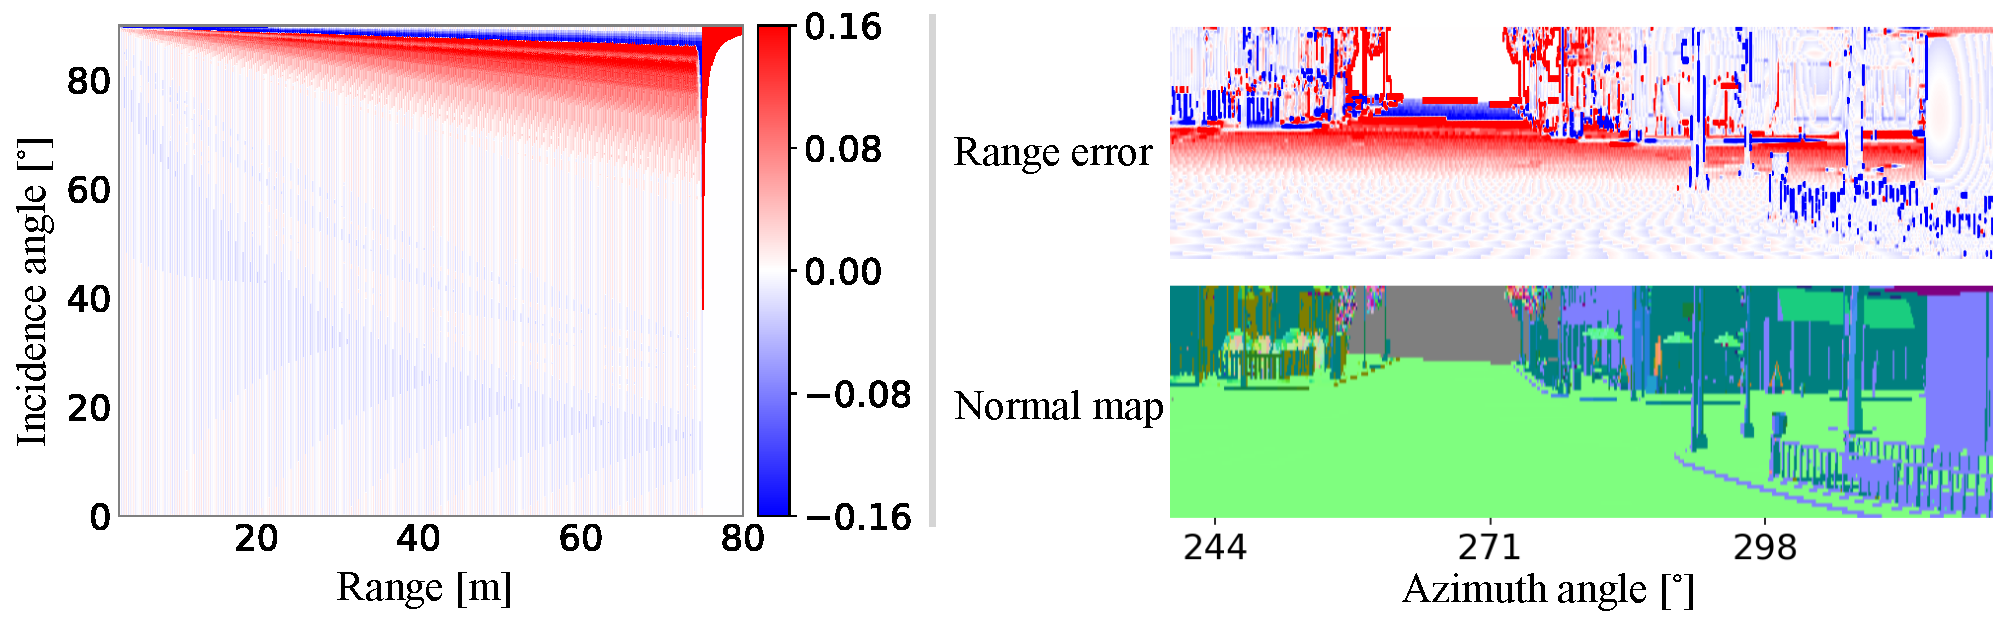
\includegraphics[width=1.0\columnwidth]{main/images/toy_example_update.pdf}
\caption{The range accuracy of the LiDAR sensor is affected by waveform discretization and beam divergence. %
The LiDAR sensor has a tendency to overestimate range in high incidence angle regime, which becomes increasingly pronounced at higher range regimes (left). This is also reflected on \textit{TownReal} dataset (right).}
\label{fig:toy_example}
\end{figure}

\section{Dynamic Neural Scene Representation}

\paragraph{Problem statement} 
Consider a set of LiDAR scans $\mathcal{X} = \{\mathbf{X}_t\}_{t=1}^T$ that have been compensated for ego-motion, along with tracked bounding boxes\footnote{We assume that the ground truth object detection and tracking annotations are available.} for dynamic vehicles $\mathcal{B} = \{\mathbf{B}_t^v\}_{v=1}^{N}$, where $T$ represents the total number of LiDAR scans, and $N$ is the count of dynamic vehicles. Each scan $\mathbf{X}_t$ is composed of $n_t$ rays, each ray $\mathbf{r}$ is described by the tuple $(\origin, \dir, \zeta, \intensity, \pdrop)$, where $\origin$ and $\dir$ denote the ray's origin and direction, $\zeta$ and $\intensity$ represent range and intensity values, and $\pdrop \in \{0,1\}$ indicates whether the ray is dropped or not due to insufficient returned radiant power.


The goal is to reconstruct the scene with a static-dynamic decomposed neural representation, that can enable the rendering of LiDAR scan $\mathbf{X}_{\text{tgt}}$ from novel viewpoint $\mathbf{T}_{\text{tgt}}$. This setup also facilitates various object manipulations, including altering object trajectories, and inserting or removing objects from the scene. The overview of our method is given in~\cref{fig:main}.

\subsection{Neural Scene Decomposition} \label{sec: decomposition}
We leverage the inductive bias that driving scenes can be decomposed into a static component and $N$ rigidly-moving dynamic components~\cite{huang2022dynamic,gojcic2021weakly}. Consequently, we establish $N+1$ neural fields. The neural field $\mathbf{F}_{\text{static}}$ is designated for the static component of the scene, capturing the unchanging background elements. Concurrently, the set of neural fields $\{\mathbf{F}^v\}_{v=1}^{N}$ is used to model the $N$ dynamic entities, specifically the vehicles in motion.



\paragraph{Neural field for static background} 
The static background is encoded into a neural field $\mathbf{F}_\text{static}: (\x, \dir) \mapsto (s, \intensity, \pdrop)$ that estimates the signed distance $s$, intensity $\intensity$, and ray drop probability $\pdrop \in [0,1]$ given the point coordinates $\x$ and the ray direction $\dir$. In practice, we first use a multi-resolution hash encoding (MRH)~\cite{mueller2022instant} to map each point to its positional feature $\posfeat \in \real^{32}$, and project the view direction onto the first 16 coefficients of the spherical harmonics basis, resulting in $\dirfeat$. Subsequently, we utilize three Multilayer Perceptrons (MLPs) to estimate the scene properties as follows:
\begin{equation}
(s, \geofeat) = f_s(\posfeat), \quad \intensity = f_{\intensity}(\rayfeat), \quad \pdrop = f_{\text{drop}}(\rayfeat).
\end{equation}
Here, $f_s, f_e,$ and $f_{\text{drop}}$ are three MLPs, $\rayfeat \in \mathbb{R}^{31}$ represents the ray feature and is constructed by concatenating the per-point geometric feature and the directional feature. The geometric feature is denoted as $\geofeat \in \mathbb{R}^{16}$. For more implementation details, please refer to the appendix. 

\begin{figure}[t]
    \centering
        \includegraphics[width=1.0\columnwidth]{Figures/overview.pdf}
        \caption{
        Overview of \dynfl. Our method takes LiDAR scans and tracked bounding boxes of dynamic vehicles as input. \dynfl first decomposes the scene into a static background and $N$ dynamic vehicles, each modelled using a dedicated neural field. These neural fields are then composed to re-simulate LiDAR scans in dynamic scenes. Our composition technique supports various scene edits, including altering object trajectories, removing and adding reconstructed neural assets between scenes.
    }
    \label{fig:main}
\end{figure}


\paragraph{Neural fields for dynamic vehicles} 
LiDAR scans collected over time are often mis-aligned due to the motion of both the sensor and other objects in the scene. Despite applying ego-motion for aligning static background points, dynamic object points remain blurred along their trajectories. Our approach to constructing a dynamic neural scene representation is grounded in the assumption that each dynamic object only undergoes rigid motion. Therefore, we can first align them over time and reconstruct them in their \textit{canonical} coordinate frame, and then render them over time by reversing the alignment of the neural field.

Specifically, consider a dynamic vehicle $v$ 
occurring in LiDAR scans $\{\mathbf{X}^v_t\}_{t=1}^{T}$ along with the associated bounding boxes $\{\mathbf{B}^v_t \in \mathbb{R}^{3\times 8}\}_{t=1}^{T}$ in the world coordinate framework. Here each bounding box is defined by its eight corners, and the first bounding box $\mathbf{B}^v_1$ is considered as the \textit{canonical} box. We estimate the relative transformations $\{\mathbf{T}_t \in \text{SE}(3)\}_{t=2}^{T}$ between the remaining $T-1$ bounding boxes and the canonical box, expressed as $\mathbf{B}_1^v = \mathbf{T}_t \mathbf{B}_t^v$\footnote{$\mathbf{T}\mathbf{B} = \mathbf{R}\mathbf{B} + \mathbf{t}$, where $\mathbf{R}$ and $\mathbf{t}$ are the rotation and translation components of $\mathbf{T}$.}. 
Subsequently, all LiDAR measurements on the object are transformed and accumulated in its canonical coordinate frame. The vehicle $v$ is then reconstructed in its canonical space, akin to the static background, using a neural field $\mathbf{F}^v$. To render the dynamic vehicle at timestamp $t$, the corresponding rigid transformation is applied to the queried rays. The dynamic neural field can thus be expressed as: $\mathbf{F}^v_t: (\mathbf{T}_{t}\x, \mathbf{T}_{t}\dir) \mapsto (s, \intensity, \pdrop)$. The rendering process for $\mathbf{F}^v$ is the same as rendering for static neural field $\mathbf{F}_{\text{static}}$.



% \section{LiDAR Novel View Synthesis}
\label{sec:method}

We now turn to constructing a neural field model tailored for LiDAR scans, along with a differentiable volume rendering scheme to enable LiDAR novel view synthesis.
We first formulate the problem setting, then set up a corresponding neural scene representation (\cref{sec:neural_scene_rep}) and derive volume rendering for active sensing (\cref{sec:lidar_vr}). Finally, we describe the rendering procedure used to synthesize novel views (\cref{sec:render_lidar}) and our optimisation scheme (\cref{sec:opt}). 


\paragraph{Problem setting}
Consider a collection of LiDAR scans $\mathcal{X} = \{\mathbf{X}_v\}_{v=1}^{n_v}$ captured by a moving sensor (\eg, mounted on a vehicle). Each scan $\mathbf{X}_v$ is associated with a sensor pose $\mathbf{T}_v \in \text{SE}(3)$ and consists of $n_r$ rays. Every ray $\ray(\origin, \dir)$ records observations $(\zeta_1, \intensity_1, \pdrop, \ptwo, \zeta_2, \intensity_2)$: the range $\zeta_1$ and intensity $\intensity_1$ of the first return; a ray drop flag $\pdrop \in \{0, 1\}$; a two-return mask $\ptwo \in \{0,1\}$; and range $\zeta_2$ and intensity~$\intensity_2$ values of the second return.
Our goal is to reconstruct a (continuous) volumetric representation of the scene in terms of density $\density$ and reflectance $\reflectance$, from which we can subsequently render virtual LiDAR scans $\mathbf{X}_{tgt}$ from novel sensor poses $\mathbf{T}_{tgt}$.

\subsection{Neural scene representation}\label{sec:neural_scene_rep}
We encode the scene as a neural field $F: (\x, \dir) \mapsto (\density, \reflectance, \pdrop)$ that takes as input a location $\x \in \real^3$ and viewing direction $\dir \in \real^3$, and returns a density $\density$, a reflectance $\reflectance$ and a ray drop probability $\pdrop$. We found it beneficial to additionally return also a local contribution $\pdrop \in [0, 1]$ to the probability of ray drop, which will be discussed below.
Technically, we use a hash encoding~\cite{mueller2022instant} to map coordinates $\x$ to positional features $\posfeat \in \real^{32}$ and project the view direction onto the first 16 coefficients of the spherical harmonics basis, $\dirfeat \in \real^{16}$. The neural field is parameterized by four Multi-Layer Perceptrons (MLPs): $[\density; \geofeat] = f_\density(\posfeat)$ regresses density and extracts an additional geometry feature $\geofeat \in \real^{15}$ that supports the other networks; $\reflectance = f_{\reflectance}(\geofeat, \dirfeat)$ regresses reflectance; $\pdrop = f_{\text{drop}}(\geofeat, \dirfeat)$ classifies whether a ray drop occurs; and  $p_s = f_{\text{sr}}(\rayfeat)$ classifies the existance of a second return. The feature $\rayfeat$ will be detailed in \cref{sec:render_lidar}.

\subsection{Volume rendering for LiDAR rays}
\label{sec:lidar_vr}
In contrast to passive sensors like cameras that rely on ambient illumination, LiDAR actively illuminates the scene and measures the back-scattered radiance. This two-way transmittance alters the volume rendering formulation. %

\paragraph{Radiant power integration}
As discussed in \cref{sec:lidar_model} 
the radiant power along a LiDAR ray is a delta function that is non-zero only at reflecting surfaces. To incorporate this forward model into the volumetric representation we combine \cref{eq:iccv_ht} and \cref{eq:iccv_hc} to obtain the 
probabilistic radiant power:
\begin{equation}
P_\zeta = C \frac{T^2_{\zeta} \cdot \density_\zeta  \reflectance_\zeta}{\zeta^2} \cos(\theta)\;,
\label{eq:iccv_radiance}
\end{equation}
where $C$ is a system constant, $\reflectance_\zeta$ is the differentiable reflectance, and $\theta$ is the incidence angle.
In a homogeneous medium with constant reflectance $\reflectance$ and density $\density$, the integrated $P(\zeta_j \rightarrow \zeta_{j+1})$ evaluates to:
\begin{equation}
     P(\zeta_j \rightarrow \zeta_{j+1}) 
     \!=\!\!\!\int_{\zeta_j}^{\zeta_{j+1}}\!\!\!\!C \frac{T^2_{\zeta_j \rightarrow \zeta} \density_\zeta \reflectance_\zeta}{\zeta^2}\!\cos(\theta_{j})\,d\zeta
     \!\approx\!\opacity_{\zeta_j} \reflectance_{\zeta_j}', 
\label{eq:iccv_lidar_rad}
\end{equation}
where we approximate $\zeta \in [\zeta_j, \zeta_{j+1}]$ by $\frac{\zeta_j + \zeta_{j+1}}{2}$, and 
\begin{equation}
    \opacity_{\zeta_j}\!=\!\frac{1}{2}\parens*{1- e^{-2\density_{\zeta_j}\delta_j}}\;,\; \reflectance_{\zeta_j}' = C \reflectance_{\zeta_j}\frac{4 \cos(\theta_j)}{(\zeta_j + \zeta_{j+1})^2}.
\end{equation}


\paragraph{Volume rendering}
The observed power at the active sensor can be evaluated by plugging \cref{eq:iccv_lidar_rad} into \cref{eq:iccv_ vol_render_nerf}: 
\begin{equation}
      P
      =\!\sum_{j=1}^N \int_{\zeta_j}^{\zeta_{j+1}}\!\!C \frac{T^2_{\zeta} \cdot \density_\zeta \reflectance_\zeta}{\zeta^2} \cos(\theta_j) \; d\zeta
      =\!\sum_{j=1}^N w_j \reflectance_{\zeta_j}',
\end{equation}
where the weights $w_j$ are now evaluated as (\cf \cref{eq:iccv_weights_nerf}):
\begin{equation}
   w_j = 2 \opacity_{\zeta_j} \cdot\prod_{k=1}^{j-1}(1 - 2 \opacity_{\zeta_k})\;.
\label{eq:iccv_lidar_weights}
\end{equation}



\subsection{Assembling the beam from multiple rays}
\label{sec:render_lidar}
Next, we apply the adapted volume rendering formulation to multiple rays within a single LiDAR beam.


\paragraph{First range estimation}
We adopt a two-stage approach to extract range values from the neural field,\footnote{Note the similarity to the detector in the instrument that first finds the peak of the waveform, then corrects for pulse shape.} as shown in \cref{fig:iccv_overview} (a).
To estimate the range for an ideal ray $\ray$, we uniformly sample $N^c$ points and query their density values, then compute the weights $\{w^c_j\}_{j=1}^{N^c}$ using \cref{eq:lidar_weights}. A coarse peak estimate $\zeta_p$ is obtained by finding the point with the highest weight along the ray: $p = \argmax_j \{w^c_j\}_{j=1}^{N^c} $. Next, we uniformly sample $N^f$ points from the local interval $\zeta_j \in [\zeta_p - \epsilon, \zeta_p + \epsilon]$. The weights $w_j^f$ at these points are recomputed and normalized to then obtain the final, refined range estimate $\zeta_f$ as:~$\zeta_f = \sum_{j=1}^{N^f} w^f_j \cdot \zeta_j\;.$



\paragraph{Second range estimation}
As discussed in~\cref{sec:lidar_model} a single LiDAR beam might have multiple returns if enough energy was reflected from surfaces further away than the first return. To capture this behavior in our scene representation, we employ \textit{truncated} volume rendering to estimate the radiant power beyond the first return (see \cref{fig:iccv_overview} (b)).

Specifically, for each beam, we first predict a two-return mask $p_s$, by classifying its features $\rayfeat = (\geofeatbar,\dirfeat,\rangefeat)$, where $\geofeatbar$ is the volume-rendered geometric feature, and $\rangefeat$ describes the standard deviation and maximum discrepancy of range estimates at the first return. Intuitively, $\geofeatbar$ describes the local geometry (\eg an edge), $\dirfeat$ encodes the relation of the beam to the geometry, and $\rangefeat$ characterizes the beam's prior interaction with the scene.

For beams that have two returns, we then perform \textit{truncated} volume rendering as follows. We first add a buffer $\xi$\footnote{The buffer $\xi$ is sensor specific and describes the minimum spacing between two distinct returns.} to the estimated range $\zeta_1$ of the first return. We then reset the transmittance $T_{\zeta_1 + \xi}$ to 1 by zeroing out the densities up to $(\zeta_1 + \xi)$ and recalculate the weights to ensure that they adhere to \cref{eq:lidar_weights}. Finally, we repeat the range estimation described above to estimate the range of the second return $\zeta_2$. Note that for beams with two returns, the estimated range $\zeta_1$ denotes the minimum range of all rays within the beam diameter, i.e. we perform volume rendering on all rays of a beam and pick the closest one as the first return. This is different from the beams with a single return where we directly use the central ray to estimate $\zeta_1$. 






\paragraph{Reflectance estimation}
At every detected surface point we can also retrieve reflectance from the neural field, using the relation $\reflectance = \sum_{j=1}^{N^f} w_j^f \cdot \reflectance_j$.


\paragraph{Ray drop probability}
In real LiDAR sensors, some emitted beams return no range measurement at all. This happens when the observed return signal has either too low amplitude or no clear peak (\cref{fig:iccv_overview} (c)). However, this effect is hard to model in a fully physics-based way,\footnote{Beyond simple thresholding, which our beam model would support.} because it depends on (usually undisclosed) details of the detection logic. We empirically observe that the ray drop probability can be learned from LiDAR measurements. To this end, we augment the neural scene representation with a dedicated variable for the local probability of \textit{not} back-scattering radiant power $\pdrop(\zeta) \in \{0, 1\}$\footnote{Please refer to the appendix for discussions on this design choice.}. 
Volume rendering integrates that quantity into a ray drop probability: $\pdrop(\ray) = \sum_{j=1}^{N_c} w_j^c\cdot p_d(\zeta_j)$.


\subsection{Training the neural LiDAR field}
\label{sec:opt}
Given a set of posed LiDAR scans, we optimise our neural field model by minimising the loss
\begin{equation}
    \mathcal{L} = \mathcal{L}_{\text{range}} + \lambda_e \mathcal{L}_{e} + \lambda_d \mathcal{L}_{d} + \lambda_s\mathcal{L}_s\;,
\label{eq:loss}
\end{equation}
consisting of a reconstruction loss $\mathcal{L}_{\text{range}}$ for range estimation, reflectance loss $\mathcal{L}_{e}$, and classification losses $\mathcal{L}_{d}$ for ray drops and $\mathcal{L}_s$ for two returns. 


\paragraph{Range reconstruction}
We add two separate losses for the coarse range $\zeta_p$ and the refined range $\zeta_f$, $\mathcal{L}_{\text{range}} = \mathcal{L}_{\text{range}}^c + \mathcal{L}_{\text{range}}^f$. For coarse range, we impose a Gaussian distribution~\cite{rematas2021urban} around the ground truth $\hat{\zeta}$, 
\begin{equation}
    \mathcal{L}_{\text{range}}^c = \frac{1}{|\mathcal{R}|} \sum_{\ray \in \mathcal{R}} \parens*{1-\!\sum_{w_j \in \mathcal{X}_c^n}\!w_j \hat{w}_j+\!\sum_{w_k \in \mathcal{X}_c^e}\!w_k^2}\;,
\end{equation}
where $\mathcal{R}$ is the set of LiDAR rays, $\mathcal{X}_c^n$ and $\mathcal{X}_c^e$ denote points sampled within and outside the interval $[\hat{\zeta}-\epsilon,\hat{\zeta}+\epsilon]$. The ground truth weight $\hat{w}_j$ is calculated by integrating the Gaussian distribution.
The range refinement loss is defined as: $\mathcal{L}_{\text{range}}^f = \frac{1}{|\mathcal{R}|} \sum_{\ray \in \mathcal{R}} |\hat{\zeta} - \zeta_f|.$


\paragraph{Reflectance reconstruction}
is optimized by minimizing an L2 loss \wrt the ground truth intensity $\hat{\intensity}$:~$\mathcal{L}_e = \frac{1}{|\mathcal{R}|} \sum_{\ray \in \mathcal{R}} (\hat{\intensity} - \intensity)^2\;.$  


\paragraph{Ray drop and dual return masks} 
are trained as classification tasks, by minimizing the combination of a binary cross entropy loss $\mathcal{L}_{bce}$ and a Lovasz loss $\mathcal{L}_{ls}$~\cite{berman2018lovasz}:
\begin{equation}
     \mathcal{L}_* = \frac{1}{|\mathcal{R}|} \sum_{\ray \in \mathcal{R}} \left(\mathcal{L}_{bce}(p_*, \hat{p_*}) + \mathcal{L}_{ls}(p_*, \hat{p_*}) \right)\;.
\end{equation}
\section{Neural rendering of the dynamic scene}
In this section, we present the methodology for rendering LiDAR scans from the neural scene representation. We begin by revisiting the density-based volume rendering formulation for active sensors~\cite{Huang2023nfl} in \cref{sec:vol_render_background}. Subsequently, we explore the extension of this formulation to SDF-based neural scene representation in \cref{sec:sdf_vol_render}. Finally, we provide a detailed discussion on rendering LiDAR measurements from individual neural fields in~\cref{sec:dynamic_nfl_rendering} and the process of composing results from different neural fields in \cref{sec:neural_fields_composition}.



\subsection{Volume rendering for active sensor} 
\label{sec:vol_render_background}
LiDAR utilizes laser beam pulses to determine the distance to the nearest reflective surface by analyzing full waveform profile of the returned radiant power. The radiant power $P(\zeta)$ from range $\zeta$ is the result of a convolution between the pulse power $P_e(t)$ and the impulse response $H(\zeta)$, defined as~\cite{hahner2021fog,hahner2022lidar,Huang2023nfl}:
\begin{equation}
    P(\zeta) = \int_0^{2\zeta/c} P_e(t) H(\zeta - \frac{ct}{2}) \; dt\;.
\label{eq:lidar}
\end{equation}
The impulse response $H(\zeta)$ is a product of the target and sensor impulse responses: $H(\zeta) = H_T(\zeta)\cdot H_S(\zeta)$, and the individual components are expressed as:
\begin{equation}
    H_T(\zeta) = \frac{\reflectance}{\pi} \cos(\theta) \delta(\zeta - \bar{\zeta})\;, \quad  H_s(\zeta) = \transmittance^2_{\zeta} \frac{A_e}{\zeta^2}\;,
\label{eq:ht}
\end{equation}
where $\reflectance$ represents the surface reflectance, $\theta$ denotes incidence angle, $\bar{\zeta}$ is the ground truth distance to the nearest reflective surface, $\transmittance_{\zeta}$ and $A_e$ describe the transmittance at range $\zeta$ and sensor's effective area, respectively. Due to the non-differentiability introduced by the indicator function $\delta(\zeta - \bar{\zeta})$, ~\cref{eq:lidar} is non-differentiable and is thus not suitable for solving the inverse problem. NFL~\cite{Huang2023nfl} solves it by extending it into a probabilistic formulation given by:
\begin{equation}
P(\zeta) = C \cdot \frac{T^2_{\zeta} \cdot \density_\zeta  \reflectance_\zeta}{\zeta^2} \cos(\theta)\;.
\label{eq:radiance}
\end{equation}
Here, $C$ accounts for the constant values, and $\sigma_\zeta$ represents the density at range $\zeta$. The radiant can be reconstructed using the volume rendering formulation:
\begin{equation}
      P
      =\!\sum_{j=1}^N \int_{\zeta_j}^{\zeta_{j+1}}\!\!C \frac{\transmittance^2_{\zeta} \cdot \density_\zeta \reflectance_\zeta}{\zeta^2} \cos(\theta_j) \; d\zeta
      =\!\sum_{j=1}^N w_j \reflectance_{\zeta_j}',
\label{eq:radiant_inter}
\end{equation}
where the weights $w_j = 2 \opacity_{\zeta_j} \cdot\prod_{i=1}^{j-1}(1 - 2 \opacity_{\zeta_i}).$
Here $\alpha_{\zeta_j}$ is the discrete opacity at range $\zeta_j$. Please refer to~\cite{Huang2023nfl} for more details.


\subsection{SDF-based volume rendering for active sensor} 
\label{sec:sdf_vol_render}
A neural scene representation based on probabilistic density often results in surfaces with noticeable noise due to insufficient surface regularization~\cite{wang2021neus}. To address this, we opt for a signed distance-based scene representation and establish the volume rendering formulation within the framework of an active sensor. Building upon SDF-based volume rendering for passive sensors~\cite{wang2021neus}, we compute the opaque density $\tilde{\density}_{\zeta_i}$ as follows:
\begin{equation}
\tilde{\density}_{\zeta_i} = \max\left(\frac{-\frac{{\textrm{d}}\Phi_s}{{\textrm{d}} \zeta_i}(f(\zeta_i))}{\Phi_s(f(\zeta_i))},0\right),
\label{eq:sigmoid_density}
\end{equation}
where $\Phi_s(\cdot)$ represents the Sigmoid function, $f(\zeta)$ evaluates the signed distance to the surface at range $\zeta$ along the ray $\ray$. 

Next, we substitute the density $\density$ in \cref{eq:radiant_inter} with opaque density from \cref{eq:sigmoid_density} and re-evaluate the radiant power and weights as:
\begin{equation}
      P
      =\!\sum_{j=1}^N \transmittance^2_{\zeta_j} \tilde{\alpha}_{\zeta_j} \reflectance_{\zeta_j}',\quad \tilde{w}_j = 2 \tilde{\opacity}_{\zeta_j} \cdot\prod_{i=1}^{j-1}(1 - 2 \tilde{\opacity}_{\zeta_i})\;.
\end{equation}
In this context, $\tilde{\alpha}_{\zeta_j}$ is computed as:
\begin{equation}
    \tilde{\alpha}_{\zeta_j} = \max\left(\!\frac{{\Phi_s(f(\zeta_j))}^2 -{\Phi_s(f(\zeta_{j+1}))}^2}{{2\Phi_s(f(\zeta_j))}^2},0\right).
    \label{eq:new_weights}
\end{equation}
Please refer to the appendix for more details.


\subsection{Volume rendering for LiDAR measurements}
\label{sec:dynamic_nfl_rendering}
Consider rendering the LiDAR measurements from a single neural field, we employ the hierarchical sampling\cite{wang2021neus} technique to sample a total of $N_s= N_u + N_i$ points along each ray, where $N_u$ points are uniformly sampled, and $N_i$ points are probabilistically sampled based on the weights along the ray, facilitating denser sampling in proximity to the surface. Subsequently, we compute the weights for the $N_s$ points following~\cref{eq:new_weights}. The rendering of range, intensity, and ray drop for each ray can be expressed through volume rendering as follows: $y_\text{est} = \sum_{j=1}^{N_s} w_j y_j$, where $y \in \{\zeta, \intensity, \pdrop\}$.


\subsection{Neural rendering for multiple fields}\label{sec:neural_fields_composition}
Our full neural scene representation comprises $N+1$ neural fields as discussed in ~\cref{sec: decomposition}. Rendering from all these fields for each ray during inference is computationally intensive. To address this, we implement a two-stage method. In the first stage, we identify the $k+1$ neural fields, where $k \geq 0$ represents the number of dynamic fields, that are likely to intersect with a given ray. The second stage involves rendering LiDAR measurements from these selected fields individually and then integrating them into a unified set of measurements.


\paragraph{Ray intersection test}
As outlined in~\cref{sec: decomposition}, each dynamic neural field is reconstructed in its unique canonical space, defined by a corresponding canonical box. To determine neural fields intersecting with a ray at inference time, we begin by estimating the transformations $\{\mathbf{T}_t^v\}_{v=1}^N$, which convert coordinates from the world framework to each vehicle's canonical space at timestamp $t$. These transformations are determined by interpolating the training set transformations using spherical linear interpolation (SLERP)~\cite{10.1145/325334.325242}. Following this, we apply transformations to the queried ray and run intersection tests with the canonical boxes of the scenes. 


\paragraph{Neural rendering from multiple neural fields}
 After identifying the $k+1$ neural fields that potentially intersect with a ray, we perform volume rendering on each field separately, yielding $k+1$ distinct sets of LiDAR measurements. Next, we evaluate the ray drop probabilities across these fields. A ray is deemed \textit{dropped} if all neural fields indicate a drop probability $\pdrop > 0.5$. For rays not classified as dropped, we sort the estimated ranges in ascending order and select the nearest one as our final range prediction. Correspondingly, the intensity value is extracted from the same neural field associated with this closest range.

\section{Neural Scene Optimisation} \label{sec:optmisation}
Given the set of LiDAR scans and the associated tracked bounding boxes of the dynamic vehicles, we optimise our neural scene representation by minimising the loss:
\begin{equation}
    \mathcal{L} = w_{\zeta} \mathcal{L}_{\zeta} +  w_{s} \mathcal{L}_{s} + w_{\text{eik}} \mathcal{L}_{\text{eik}} + w_{\intensity} \mathcal{L}_{\intensity} + w_{\text{drop}} \mathcal{L}_{\text{drop}},
    \label{loss}
\end{equation}
where $w_{*}$ denotes respective weights, and each individual loss term $\mathcal{L}_*$ is explained below.


\paragraph{Range reconstruction loss}
For range estimation, we employ L1 loss, defined as: $\mathcal{L}_{\zeta} = \frac{1}{|\mathcal{R}|}\sum_{\ray \in \mathcal{R}}|\zeta_{est} -\zeta_{gt}|$, where $\mathcal{R}$ denotes the set of LiDAR rays, $\zeta_{est}$ and $\zeta_{gt}$ correspond to the estimated and actual ranges, respectively. 


\paragraph{Surface points' SDF regularisation} \label{sec:surfacesdf}
Acknowledging that LiDAR points mostly come from actual surface, we introduce an additional SDF regularisation term $\mathcal{L}_{s}$ that penalizes surface points' SDF values: $\mathcal{L}_{s} = \frac{1}{|\mathcal{P}|}\sum_{\mathbf{p} \in \mathcal{P}}|s(\mathbf{p})|$. Here $\mathcal{P}$ denotes the set of surface points and $s({\mathbf{p}})$ represents the SDF value of the point $\mathbf{p}$.


\paragraph{Eikonal constraint}
Following~\cite{icml2020_2086}, we utilize the Eikonal loss, $\leik$, to regularize the SDF level set. This ensures the gradient norm of the SDF is approximately one at any queried point. The loss is computed as: $\leik = \frac{1}{|\mathcal{Z}|} \sum_{\mathbf{p} \in \mathcal{Z}}( \| \nabla s(\mathbf{p}) \|_2 - 1)^2$, where $\mathcal{Z}$ is the set of all the sampled points. To stablise the training procedure, we adopt a numerical approach~\cite{li2023neuralangelo} to compute $\nabla s(\pos)$ as: 
\begin{equation}
    \nabla s(\pos) = \frac{s \left( \pos + \boldsymbol{\epsilon} \right) - s \left(\pos - \boldsymbol{\epsilon} \right)}{2 \epsilon} \;,
    \label{eqn:central_diff_normal}
\end{equation}
where the numerical step size $\epsilon$ is set to be $10^{-3}$ meters.


\paragraph{Intensity Loss}
For intensity reconstruction, we apply L2 loss, defined as: $\mathcal{L}_{\intensity} = \frac{1}{|\mathcal{R}|}\sum_{\ray \in \mathcal{R}}(\intensity_{est} -\intensity_{gt})^2.$


\paragraph{Ray drop loss}
We follow~\cite{Huang2023nfl} to supervise the ray drop estimation with a combination of a binary cross entropy loss $\mathcal{L}_{bce}$ and a Lovasz loss $\mathcal{L}_{ls}$ \cite{berman2018lovasz} as:
\begin{equation}
     \mathcal{L}_{\text{drop}} = \frac{1}{|\mathcal{R}|} \sum_{\ray \in \mathcal{R}} \left(\mathcal{L}_{bce}(p_{d, est}, {p_{d, gt}}) + \mathcal{L}_{ls}(p_{d, est}, {p_{d, gt}}) \right)\;.
     \label{eq:raydrop_loss}
\end{equation}
It's worth noting that in the context of dynamic neural fields, during training, we incorporate all LiDAR rays that intersect with the objects' bounding boxes of the scenes. A ray is classified as \textit{dropped} either if it is labeled as such in the dataset or if it does not intersect with the actual surfaces of the dynamic vehicles (\eg rays that are close but in parallel to the surfaces). This approach enhances the accuracy and realism of the reconstructed dynamic neural fields, improving the rendering fidelity at inference time. 

\section{Experiments}
\begin{figure*}[t]
  \centering
   \includegraphics[width=1\textwidth]{Figures/errormap_dynamic_3.pdf}
   
   \caption{Qualitative comparison of range estimation on \textit{Waymo Dynamic} dataset. Dynamic vehicles are zoomed in, and points are color-coded by range errors~(-100 \bwrDyNFL~100 cm).
   }
   \label{fig:errormap_dynamic}
   
\end{figure*}








\subsection{Datasets and Evaluation Protocol}\label{sec:datasets}

\paragraph{Real-world dynamic scenes} 
We construct \textit{Waymo Dynamic} dataset by selecting four representative scenes from Waymo Open dataset~\cite{sun2020scalability}, with multiple moving vehicles inside. These scenes are comprised of sequences of 50 consecutive frames. For evaluation purposes, every fifth frame is designated for testing, while the other 40 frames are allocated for training.


\paragraph{Real-world static scenes}
We also evaluate our method on four static scenes as introduced in~\cite{Huang2023nfl}. There are two settings, \textit{Waymo Interp} applies the same evaluation protocol as \textit{Waymo Dynamic}, while \textit{Waymo NVS} employs a dedicated closed-loop evaluation to validate the real novel view synthesis performance. Please refer to NFL~\cite{Huang2023nfl} for more details about this setting. 
 


\paragraph{Synthetic static scenes}  
\textit{TownClean} and \textit{TownReal} are synthetic static scenes introduced in NFL~\cite{Huang2023nfl}. They consist of 50 LiDAR scans simulated in urban street environment, using non-diverging and diverging beams, respectively. 



\paragraph{Evaluation metrics}\label{sec:metrics}
To evaluate the LiDAR range accuracy, we employ a suite of four metrics: mean absolute errors~(MAE [cm]), median absolute errors~(MedAE [cm]), Chamfer distance~(CD[cm]) and MedAE for dynamic vehicles~(MedAE Dyn[cm]). For intensity evaluation, We report root mean square error~(RMSE).
%
In addition to our primary evaluations, we assess the re-simulated LiDAR scans' realism through two auxiliary tasks: object detection and semantic segmentation. For object detection, we calculate the \textit{detection agreement}~\cite{manivasagam2020lidarsim}, both for all vehicles (Agg.~[\%]) and specifically for dynamic vehicles (Dyn.$\;$Agg.~[\%]). Regarding semantic segmentation, we measure and report recall, precision, and the intersection over union (IoU[\%]). It's important to note that the predictions on the original LiDAR scans serve as our \textit{ground truth}, against which we compare the results obtained from the re-simulated scans.




\paragraph{Baseline methods}
Regarding LiDAR simulation on static scenes, NFL~\cite{Huang2023nfl} and LiDARsim\cite{manivasagam2020lidarsim} are two closest baselines to compare to. Additionally, we include i-NGP~\cite{mueller2022instant}, DS-NeRF~\cite{kangle2021dsnerf}, and URF~\cite{rematas2022urban} for comparison. As for simulation on dynamic scenes, we compare to LiDARsim~\cite{manivasagam2020lidarsim} and UniSim~\cite{yang2023unisim}\footnote{We re-implement LiDARsim~\cite{lee2015lidar} and UniSim~\cite{yang2023unisim} as they are not open-sourced.}. Please refer to the appendix for implementation details.


\begin{table}[t]
    \setlength{\tabcolsep}{4pt}
    \renewcommand{\arraystretch}{1.2}
	\centering
	\resizebox{\columnwidth}{!}{
    \begin{tabular}{l|ccccc}
    \toprule
    Method  & MAE $\downarrow$ &  MedAE $\downarrow$ & CD $\downarrow$ & MedAE Dyn $\downarrow$ & Intensity RMSE $\downarrow$\\
    \midrule
    LiDARsim~\cite{manivasagam2020lidarsim} & 170.1 & 11.5 & 31.1 &  16.0  & 0.10\\
    Unisim~\cite{yang2023unisim} & 35.6 & 6.1 & 14.3 &14.3 & \textbf{0.05}\\
    Ours~ & \textbf{30.8} & \textbf{3.0} & \textbf{10.9} &\textbf{8.5} & \textbf{0.05}\\
    \bottomrule
    \end{tabular}
    }
    
	\caption{Evaluation of LiDAR NVS on \textit{Waymo Dynamic} dataset.}
	\label{tab:waymodynamic}
\end{table}
\begin{table}[t]
    \setlength{\tabcolsep}{4pt}
    \renewcommand{\arraystretch}{1.2}
	\centering
	\resizebox{\columnwidth}{!}{
    \begin{tabular}{l|ccc|ccc|ccc|ccc}
    \toprule
    & \multicolumn{3}{c|}{TownClean}& \multicolumn{3}{c|}{TownReal} & \multicolumn{3}{c|}{Waymo interp.} & \multicolumn{3}{c}{Waymo NVS} \\
    Method  & MAE $\downarrow$ &  MedAE $\downarrow$ & CD $\downarrow$& MAE $\downarrow$ &  MedAE $\downarrow$ & CD $\downarrow$ & MAE $\downarrow$ &  MedAE $\downarrow$ & CD $\downarrow$ & MAE $\downarrow$ &  MedAE $\downarrow$ & CD $\downarrow$\\
    \midrule
    i-NGP~\cite{mueller2022instant} &42.2 &4.1 & 17.4 & 49.8 & 4.8 & 19.9 & \textbf{26.4} & 5.5 & \textbf{11.6} & \underline{30.4} & 7.3 & 15.3\\
    DS-NeRF~\cite{kangle2021dsnerf} &41.7 & 3.9 &16.6 & 48.9 & 4.4 & 18.8 & \underline{28.2} & 6.3 & 14.5 & 30.4 & 7.2 & 16.8 \\
    URF~\cite{rematas2022urban} &43.3&4.2&16.8& 52.1 & 5.1 & 20.7 & 28.2 & 5.4 & 12.9 & 43.1 & 10.0 & 21.2 \\
    LiDARsim~\cite{manivasagam2020lidarsim} &159.6&\underline{0.8}&23.5& 162.8 & 3.8 & 27.4 & 116.3 & 15.2 & 27.6 & 160.2 & 16.2 & 34.7 \\
    NFL\cite{Huang2023nfl}  &\underline{32.0}&2.3&\underline{9.0}& \underline{39.2} & \underline{3.0} & \underline{11.5} & 30.8 & \underline{5.1} & \underline{12.1}& 32.6 & \underline{5.5} & \underline{13.2}  \\
    Ours & \textbf{26.7} & \textbf{0.7} & \textbf{6.7} &\textbf{33.9}&\textbf{2.1}&\textbf{10.4}& 28.3 & \textbf{4.7} & 12.5 & \textbf{28.6} & \textbf{4.9} & \textbf{13.0} \\
    \bottomrule
    \end{tabular}
}
    
	\caption{Evaluation of LiDAR NVS on static scenes.}
	\label{tab:waymostatic}
\end{table}
\begin{figure}[t]
  \centering
   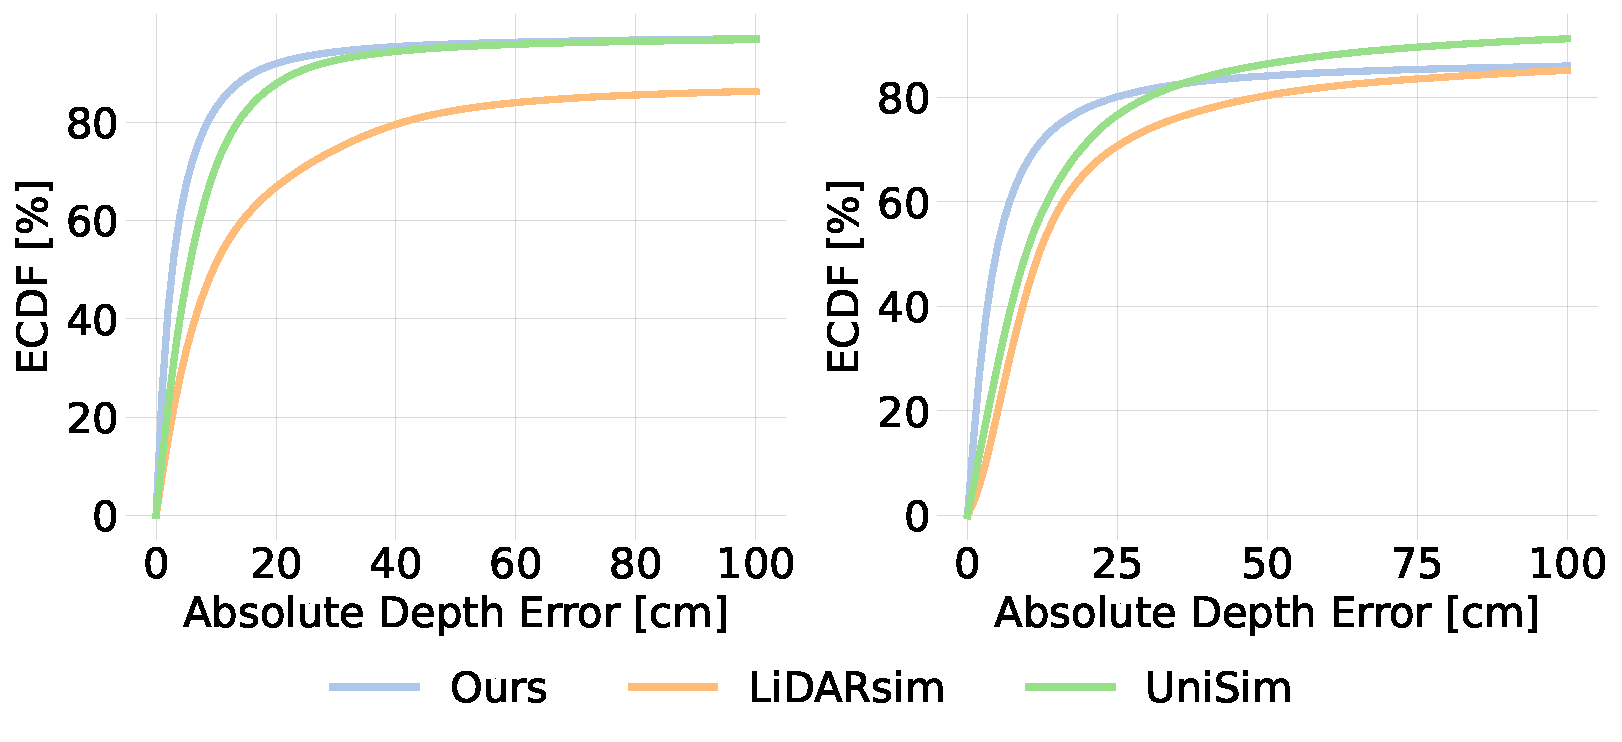
\includegraphics[width=1\columnwidth]{Figures/ecdf_3_methods.pdf}
   
        \caption{ECDF plots showcasing range errors across all the points (left) and specifically for points associated with dynamic vehicles (right). Our neural fields composition demonstrates superior performance over LiDARsim~\cite{manivasagam2020lidarsim} and UniSim~\cite{yang2023unisim}, especially in the context of dynamic vehicles.}
   \label{fig:ecdf}
   
\end{figure}
\begin{figure}[t]
    \centering
        \includegraphics[width=1\columnwidth]{Figures/errormap_static.pdf}
        
        \caption{Qualitative results of range estimation. Regions with gross errors (-100 \bwrDyNFL~100 cm) are highlighted.
        }
    \label{fig:error_map}
\end{figure}
\subsection{LiDAR Novel View Synthesis Evaluation} \label{sec:lidar_eval}
\paragraph{LiDAR NVS in dynamic scenes}
Quantitative comparisons with baseline methods are detailed in~\cref{tab:waymodynamic}. \dynfl notably outperforms LiDARsim~\cite{manivasagam2020lidarsim} and UniSim~\cite{yang2023unisim} in range reconstruction. This improvement is largely due to our SDF-based neural scene representation, which incorporates the physical aspects of LiDAR sensing. Additionally, our method employs a ray drop test when rendering multiple neural fields, leading to a more accurate reconstruction of dynamic vehicles, as evidenced in~\cref{fig:errormap_dynamic} and further supported by the data in~\cref{fig:ecdf}.


\begin{figure*}[t]
    \centering
        \includegraphics[width=1.0\textwidth]
        {Figures/sensor_manipulation.pdf}
        
        \caption{LiDAR novel view synthesis by changing sensor elevation angle~($\theta$), poses~($x,y,z$) and number of beams on \textit{Waymo Dynamic} dataset. The points are color-coded by the intensity values (0 \bwrDyNFL~0.25).}
    \label{fig:lidar_nvs}
\end{figure*}
\paragraph{LiDAR NVS in static scenes}
In addition to dynamic scenes, we evaluate \dynfl against baseline methods in static scenarios, with the results detailed in~\cref{tab:waymostatic} and~\cref{fig:error_map}. \dynfl excels in reconstructing geometry in most cases. A key observation is its superior performance in reconstructing planar regions (\eg the ground shown in~\cref{fig:error_map}), especially when compared to NFL~\cite{Huang2023nfl}, which also uses a neural field for surface representation. This improvement is largely due to the enhanced surface regularizations provided by our advanced SDF-based surface modeling approach.


\begin{table}[t]
    \setlength{\tabcolsep}{4pt}
    \renewcommand{\arraystretch}{1.2}
	\centering
	\resizebox{0.5\columnwidth}{!}{
    \small
    \begin{tabular}{l|ccc}
    \toprule
    Datasets  & MAE $\downarrow$ &  MedAE $\downarrow$ & CD $\downarrow$ \\
    \midrule
    TownClean~ & 26.7(\textcolor{green}{-1.5}) & 0.7(\textcolor{green}{-0.2}) & 6.7(\textcolor{green}{-0.5})\\
    Waymo Interp~ & 28.3 (\textcolor{red}{0.1}) & 4.7 (\textcolor{green}{-0.2}) & 12.5 (\textcolor{green}{-0.1})\\
    Waymo Dynamic~ & 30.8 (\textcolor{green}{-0.3}) & 3.0 (\textcolor{green}{-0.2}) & 10.9 (\textcolor{green}{-0.3})\\
    \bottomrule
    \end{tabular}
    }
    
	\caption{Ablation study of volume rendering for active sensing.}
	\label{tab:active_sensing}
\end{table}
\begin{table}[t]
    \setlength{\tabcolsep}{4pt}
    \renewcommand{\arraystretch}{1.2}
	\centering
	\resizebox{0.5\columnwidth}{!}{
    \small
    \begin{tabular}{l|ccc}
    \toprule
    Datasets  & MAE $\downarrow$ &  MedAE $\downarrow$ & CD $\downarrow$ \\
    \midrule
    TownReal~ & 33.9(\textcolor{green}{-3.3}) & 2.1(\textcolor{green}{-0.0}) & 10.4(\textcolor{green}{-1.2})\\
    Waymo Interp~ & 28.3 (\textcolor{green}{-0.3}) & 4.7 (\textcolor{green}{-0.1}) & 12.5 (\textcolor{green}{-0.3})\\
    \bottomrule
    \end{tabular}
    }
    
	\caption{Ablation study of the surface points' SDF regularisation.}
	\label{tab:surface_sdf}
\end{table}
\begin{figure}[t]
  \centering
   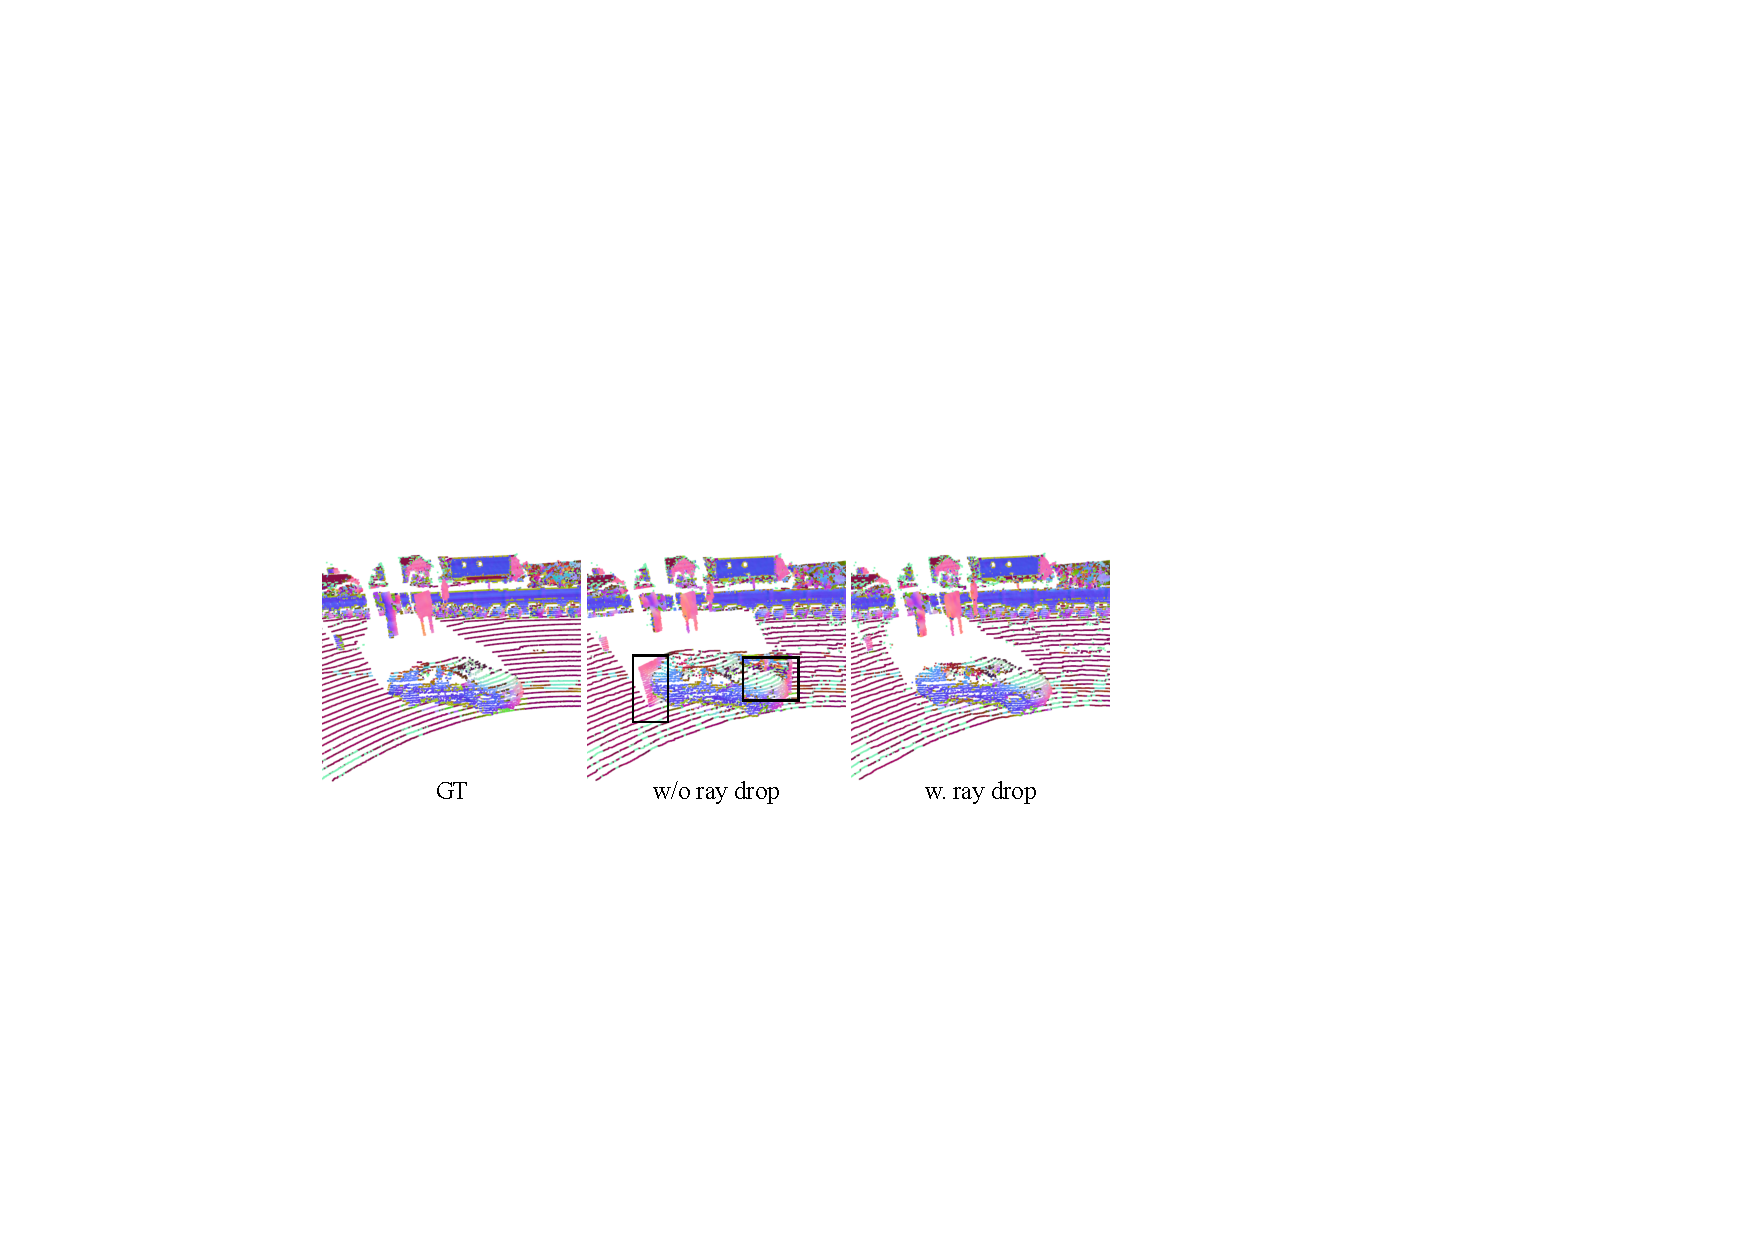
\includegraphics[width=1\linewidth]{Figures/intersectiontest.pdf}
   
   \caption{
   Qualitative results on \textit{Waymo Dynamic} dataset. Our model equipped with a ray drop module effectively composites multiple neural fields, re-simulating LiDAR scans of high quality.
   }
   % \caption{These figures exemplify the effectiveness of our field composition method leveraging ray drop probability from dynamic neural field. When all intersected rays are rendered for the dynamic neural field, noticeable artifacts appear due to disturbances from irrelevant fields (middle figure). The figures on the right showcase the complete composition method.
   % }
   % \caption{
   % }
    
   \label{fig:ablation_raydrop}
\end{figure}

\begin{figure}[t]
    \centering
        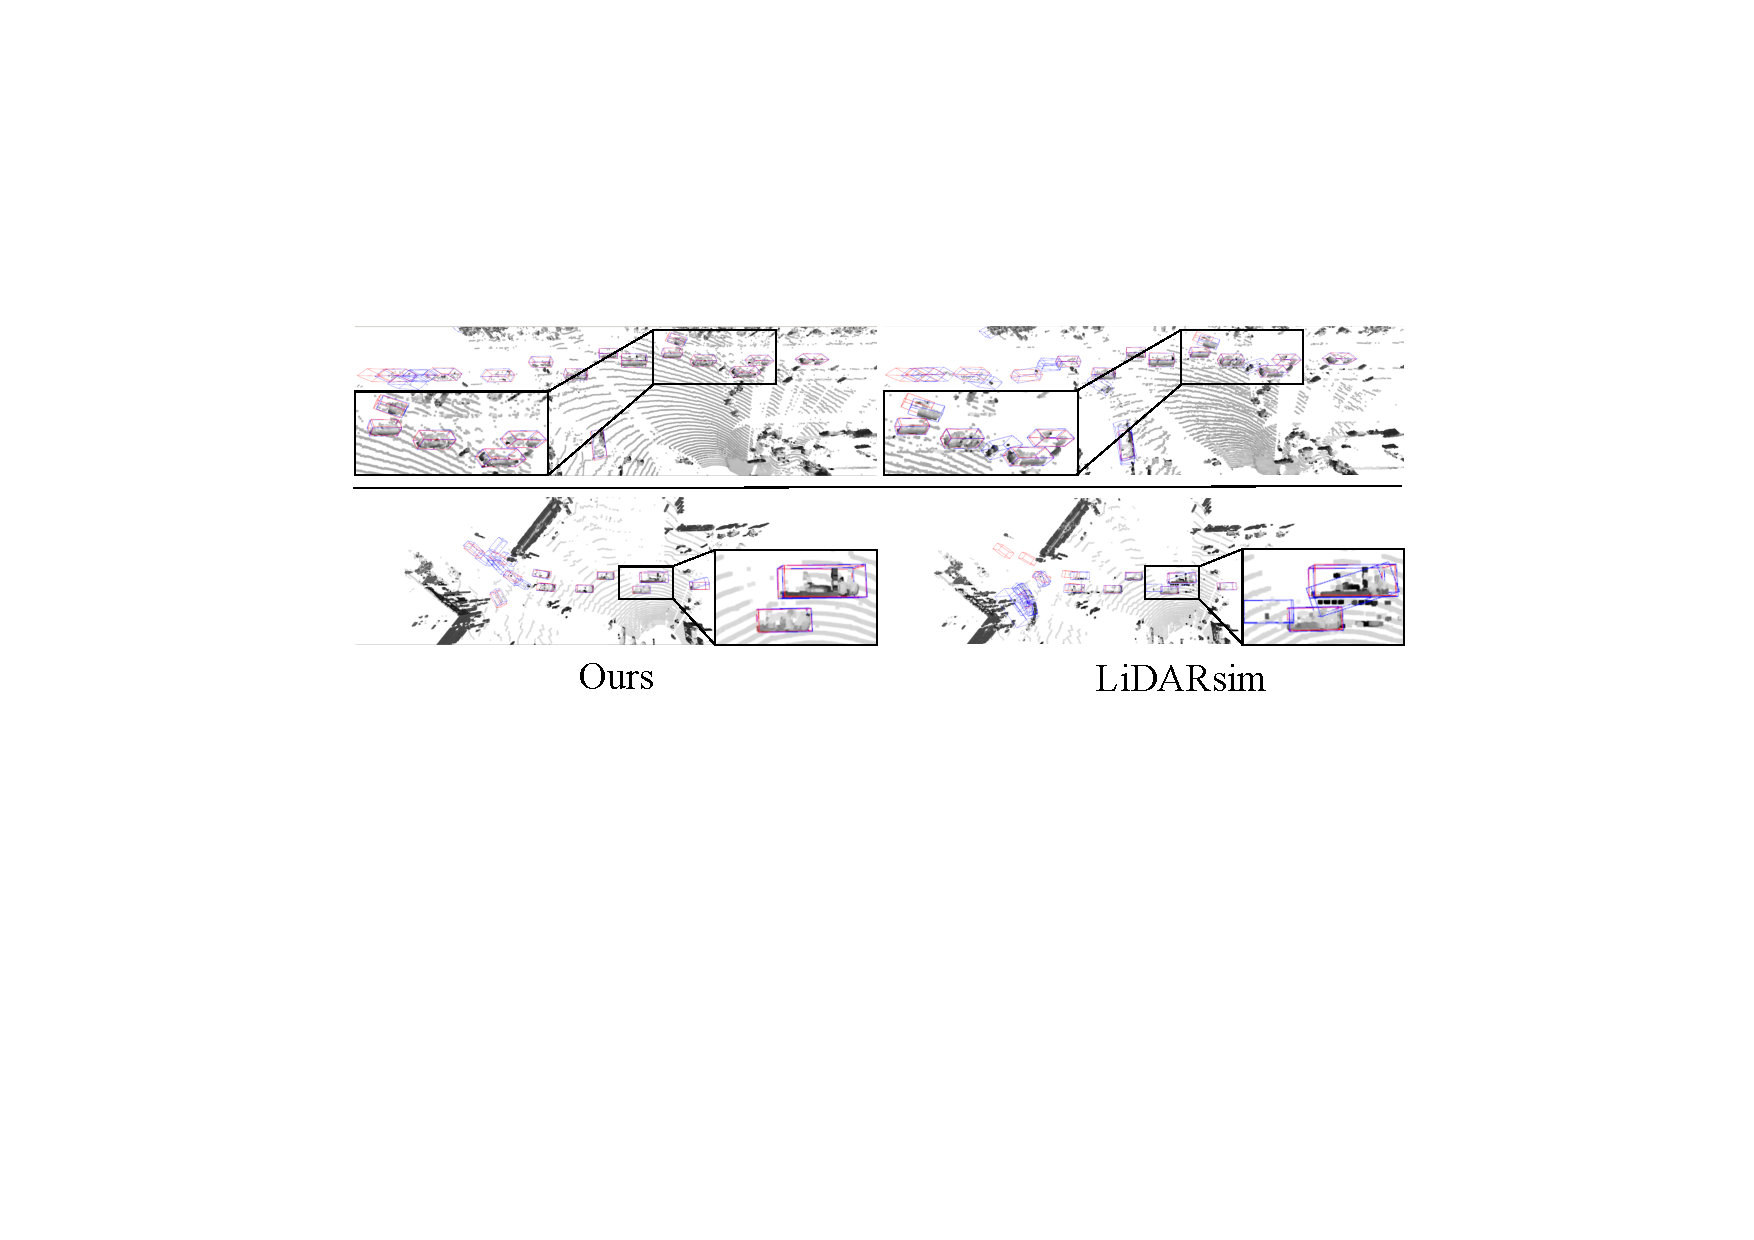
\includegraphics[width=0.8\columnwidth]{Figures/detection_result.pdf}
        \caption{Object detection results on \textit{Waymo Dynamic} dataset. The ground truth and predicted bounding boxes are marked in \textcolor{red}{red} and \textcolor{blue}{blue}, respectively.}
    \label{fig:detection}
    
\end{figure}
% \begin{table}[t]
% 	\centering
% 	\resizebox{0.8\columnwidth}{!}{
% 		\begin{tabular}{@{}lcccccccc@{}}
% 			\toprule
%              & \multicolumn{1}{c}{GT} & \multicolumn{3}{c}{Ours} & \multicolumn{3}{c}{LiDARSim\cite{manivasagam2020lidarsim}} \\
% 			  \cmidrule(r){2-2}\cmidrule(r){3-5} \cmidrule(l){6-8}
% 			Threshold & AP$\uparrow$ & \multicolumn{1}{c}{AP$\uparrow$}& \multicolumn{1}{c}{Agg.$\uparrow$}& \multicolumn{1}{c}{Dyn. Agg.$\uparrow$} & \multicolumn{1}{c}{AP$\uparrow$} & \multicolumn{1}{c}{Agg.$\uparrow$}& \multicolumn{1}{c}{Dyn. Agg.$\uparrow$} \\
% 			\midrule
% 			IoU$>$0.7 &0.85  &0.86 & \textbf{0.77}& \textbf{0.71}& \textbf{0.90} & 0.76 & 0.68\\
% 			IoU$>$0.5 &\textbf{0.98}  & 0.96 & \textbf{0.87}& \textbf{0.76}& 0.95 & 0.86& \textbf{0.76} \\
% 			\bottomrule
% 		\end{tabular}
% 	}
% 	\caption{Object detection results on \textit{Waymo Dyanmic} datasets.}
    
% 	\label{tab:detection}
% \end{table}

\begin{table}[t]
	\centering
		\begin{tabularx}{\columnwidth}{l|YYYYYYY}
			\toprule
             & \multicolumn{1}{c}{GT} & \multicolumn{3}{c}{Ours} & \multicolumn{3}{c}{LiDARSim\cite{manivasagam2020lidarsim}} \\
			  \cmidrule(r){2-2}\cmidrule(r){3-5} \cmidrule(l){6-8}
			Threshold & AP$\uparrow$ & \multicolumn{1}{c}{AP$\uparrow$}& \multicolumn{1}{c}{Agg.$\uparrow$}& \multicolumn{1}{c}{Dyn. Agg.$\uparrow$} & \multicolumn{1}{c}{AP$\uparrow$} & \multicolumn{1}{c}{Agg.$\uparrow$}& \multicolumn{1}{c}{Dyn. Agg.$\uparrow$} \\
			\midrule
			IoU$>$0.7 &0.85  &0.86 & \textbf{0.77}& \textbf{0.71}& \textbf{0.90} & 0.76 & 0.68\\
			IoU$>$0.5 &\textbf{0.98}  & 0.96 & \textbf{0.87}& \textbf{0.76}& 0.95 & 0.86& \textbf{0.76} \\
			\bottomrule
		\end{tabularx}
	\caption{Object detection results on \textit{Waymo Dyanmic} datasets.}
    
	\label{tab:detection}
\end{table}
% \begin{table}[t]
% \setlength{\tabcolsep}{4pt}
% \renewcommand{\arraystretch}{1.2}
% \centering
% \resizebox{0.8\columnwidth}{!}{
% \begin{tabular}{l|ccc|ccc}
% \toprule
% & \multicolumn{3}{c|}{Vehicle} & \multicolumn{3}{c}{Background} \\
% Method & Recall $\uparrow$ & Precision $\uparrow$ & IoU $\uparrow$ & Recall $\uparrow$ & Precision $\uparrow$ & IoU $\uparrow$ \\
% \midrule
% i-NGP~\cite{muller2022instant} & \underline{93.2} & 85.9 & 80.9 & 98.3 & \underline{99.2} & 97.6\\
% DS-NeRF~\cite{deng2021depth} & 90.7 & \underline{87.1} & 80.2 & \underline{98.5} & 98.9 & 97.4\\
% URF~\cite{rematas2021urban} & 87.8 & 81.7 & 73.7 & 98.0 & 98.4 & 96.5\\
% Lidarsim~\cite{manivasagam2020lidarsim} & 90.5 & 70.5 & 65.9 & 94.9 & 99.0 & 94.0\\
% NFL density~\cite{Huang2023nfl}& \textbf{95.9} & 87.0 & \textbf{83.9} & 98.3 & \textbf{99.5} & \textbf{97.8}\\
% Ours & 90.5 & \textbf{89.2} & \underline{82.3} & \textbf{98.8} & 98.9 & \underline{97.7}\\
% \bottomrule
% \end{tabular}
% }
% 
% \caption{Semantic segmentation results on \textit{Waymo NVS} dataset.}
% \label{tab:sem_seg_nvs}
% \end{table}



\begin{table}[t]
\setlength{\tabcolsep}{4pt}
\renewcommand{\arraystretch}{1.2}
\centering
\resizebox{0.99\columnwidth}{!}{
\begin{tabular}{l|ccc|ccc}
\toprule
& \multicolumn{3}{c|}{Vehicle} & \multicolumn{3}{c}{Background} \\
Method & Recall $\uparrow$ & Precision $\uparrow$ & IoU $\uparrow$ & Recall $\uparrow$ & Precision $\uparrow$ & IoU $\uparrow$ \\
\midrule
i-NGP~\cite{mueller2022instant} & 91.8 & 83.6 & 78.1 & 97.9 & 99.2 & 97.1\\
DS-NeRF~\cite{kangle2021dsnerf} & 89.3 & 84.8 & 77.3 & 98.1 & 98.8 & 97.0\\
URF~\cite{rematas2021urban} & 86.9 & 79.8 & 72.0 & 97.7 & 98.5 & 96.2\\
Lidarsim~\cite{manivasagam2020lidarsim} & 89.6 & 68.9 & 64.0 & 94.5 & 98.9 & 93.5\\
NFL~\cite{Huang2023nfl}& \textbf{94.5} & 84.8 & 80.9 & 97.8 & \textbf{99.4} & \textbf{97.3}\\
Ours & 90.5 & \textbf{88.4} & \textbf{81.1} & \textbf{98.5} & 98.7 & \textbf{97.3}\\
\bottomrule
\end{tabular}
}

\caption{Semantic segmentation results on \textit{Waymo NVS} dataset.}
\label{tab:sem_seg_nvs_ours}

\end{table}




\subsection{Ablation Study}
\paragraph{SDF-based volume rendering for active sensing}
We begin by assessing the efficacy of our SDF-based volume rendering for active sensor, the results are shown in~\cref{tab:active_sensing}. When compared to our baseline that uses the SDF-based volume rendering for passive sensing, \dynfl demonstrates enhanced performance in both synthetic (\textit{TownClean}) and real-world (\textit{Waymo Interp} and \textit{Waymo Dynamic}) datasets, indicating the importance of incorporating the physical sensing process of LiDAR in addressing the inverse problem.


\paragraph{Neural fields composition} 
To validate the efficacy of our two-stage neural field composition approach, we compare it with an alternative approach utilized in UniSim~\cite{yang2023unisim}. The results are shown in~\cref{tab:waymodynamic}. UniSim~\cite{yang2023unisim} blends different neural fields by sampling points from all intersected neural fields, followed by a single evaluation of volume rendering to produce the final LiDAR scan. In contrast, our method independently renders from each intersecting neural field first, and then combines these measurements into a final measurement using a ray drop test (\cf~\cref{fig:ablation_raydrop}). This approach leads to a notable improvement in geometry reconstruction over UniSim~\cite{yang2023unisim}, exemplified by our method halving the Median Absolute Error (MedAE) across all points. This enhancement is even more evident when focusing solely on points related to dynamic vehicles (\cf~\cref{fig:ecdf}).
% 

\paragraph{Surface points' SDF constraint}
We examine the importance of the surface points' SDF constraint discussed in ~\cref{sec:optmisation} on \textit{Town Real} and \textit{Waymo Interp} datasets. The results shown in \cref{tab:surface_sdf} suggest that our method yields improved geometry reconstruction quality by additionally enforcing LiDAR points to have zero SDF values. 


\subsection{Auxiliary Task Evaluations} 
\label{sec:downstream}
To assess the fidelity of our neural re-simulation and gauge the domain gap between re-simulated and real scans, we evaluate their applicability in two downstream tasks: object detection and semantic segmentation.


\paragraph{Object detection}
We utilize the pre-trained FSDv2~\cite{fan2023fsdv2} model for object detection and conduct evaluations on the re-simulated LiDAR scans within the \textit{Waymo Dynamic} dataset. Our results are compared against those from LiDARsim~\cite{manivasagam2020lidarsim}, with the findings detailed in~\cref{tab:detection} and~\cref{fig:detection}. Notably, \dynfl exhibits a more substantial detection agreement with the predictions on real LiDAR scans. This indicates a higher fidelity in our re-simulations and a reduced domain gap relative to actual scans.


\paragraph{Semantic segmentation}
For semantic segmentation, we use the pre-trained SPVNAS model~\cite{tang2020searching}, with the results presented in~\cref{tab:sem_seg_nvs_ours}. \dynfl improves over baseline methods according to most evaluation metrics, underscoring the realism of our re-simulated LiDAR scans.



\subsection{Scene Editing}
Beyond LiDAR novel view synthesis by adjusting the sensor configurations (\cf \cref{fig:lidar_nvs}), we additionally demonstrate the practicality of our compositional neural fields approach through two scene editing applications.

\begin{figure}[t]
    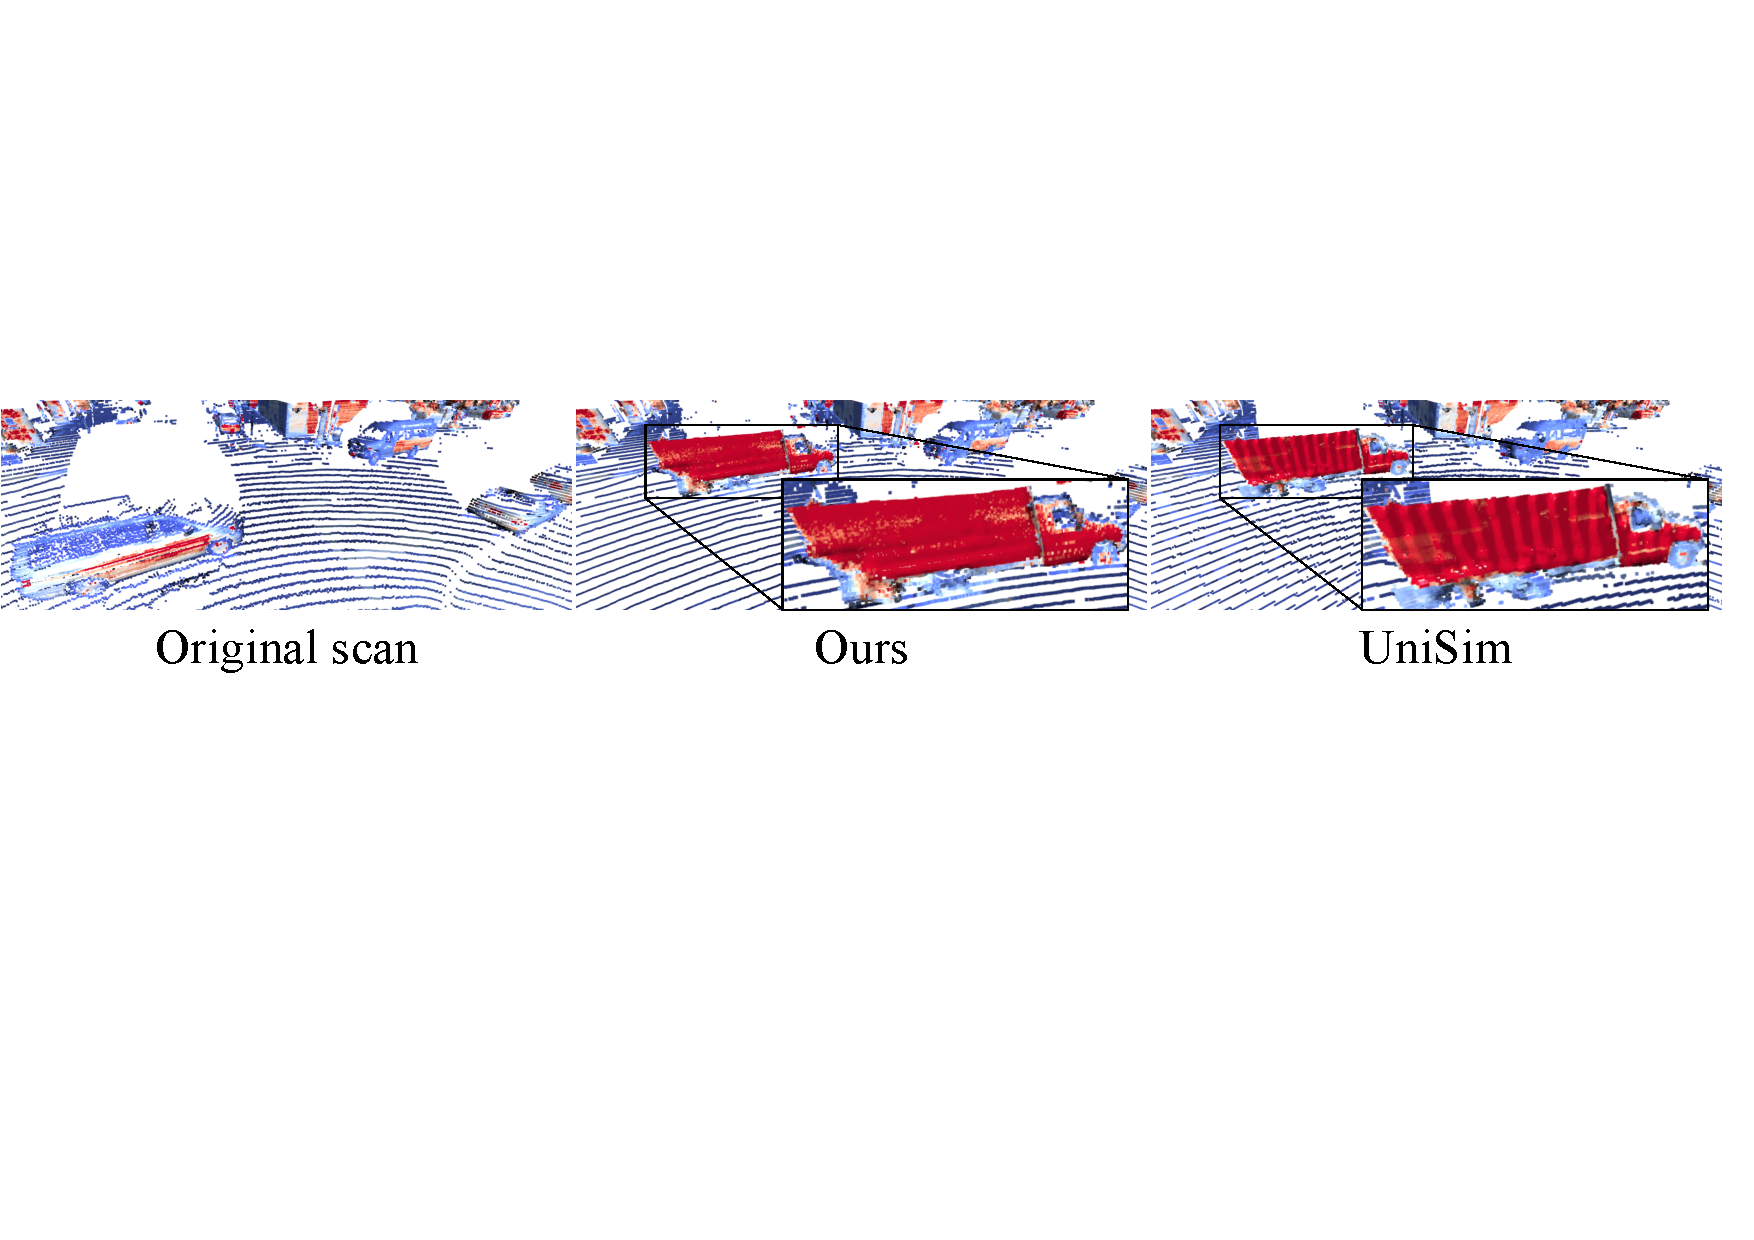
\includegraphics[width=1.0\linewidth]{Figures/vehicle_insertion.pdf}
    
    \caption{
    Qualitative results of object removal and insertion. \dynfl seamlessly inserts the neural asset (truck) into a new scene attributed to our superior compositional rendering scheme. In contrast, UniSim~\cite{yang2023unisim} struggles to accurately model geometry.
    }
    \label{fig:vehicle_insertion}
\end{figure}
\paragraph{Insert object from one scene into another}
Our explicit neural scene de-composition and flexible composition technique enable seamless insertion and removal of neural assets across scenes. As demonstrated in~\cref{fig:vehicle_insertion}, we are able to replace a car from one scene with a truck from another scene, achieving accurate reconstruction of both geometry and intensity. In contrast, UniSim~\cite{yang2023unisim} struggles to preserve high quality geometry. This highlights the significant potential of our approach in generating diverse and realistic LiDAR scans for autonomous driving scenarios.

\begin{figure}[t]
    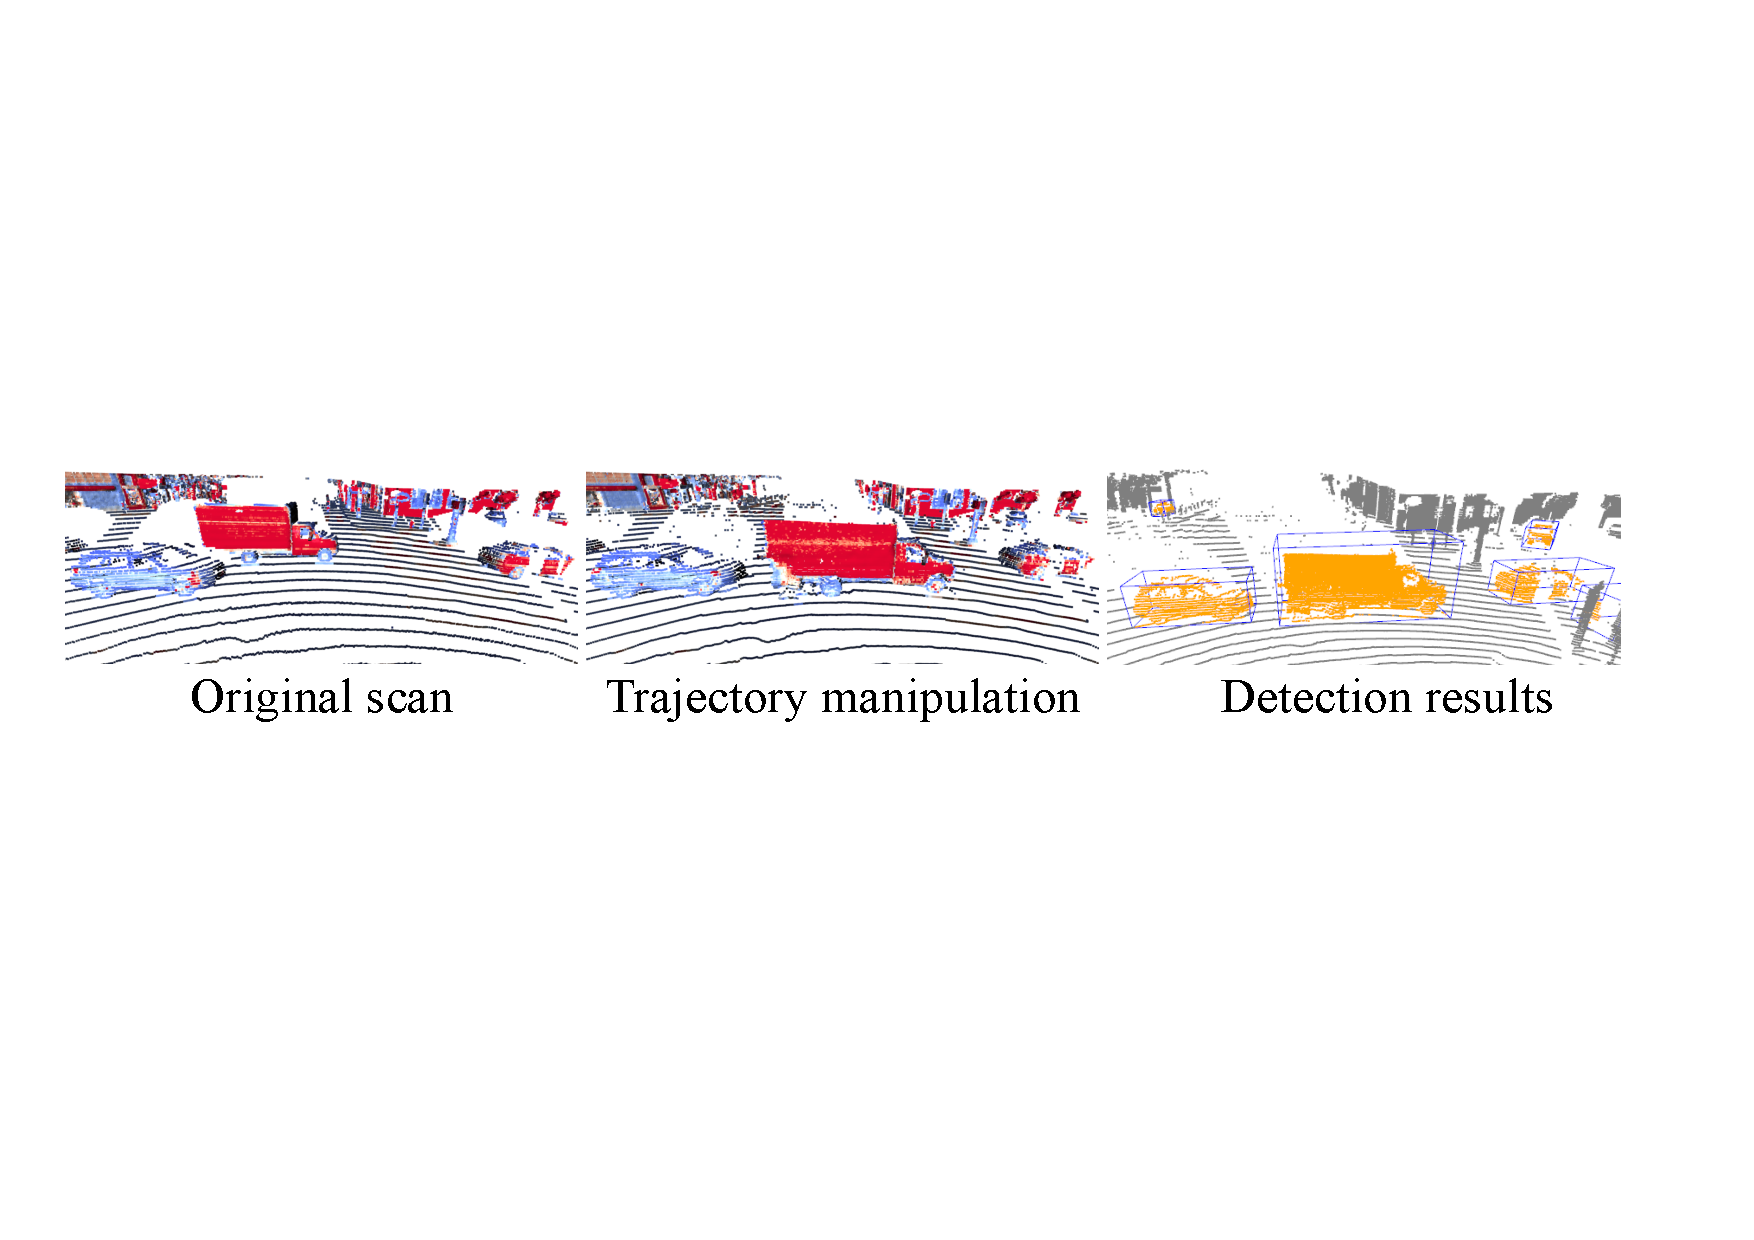
\includegraphics[width=1.0\columnwidth]{Figures/trajectory_manipulation.pdf}
    
    \caption{Qualitative results of object trajectory manipulation. The truck can be successfully detected after manipulation, indicating high-realism LiDAR re-simulation achieved by \dynfl.}
    \label{fig:traj}
    
\end{figure}
\paragraph{Manipulate the trajectory of dynamic objects}
\dynfl also facilitates the manipulation of moving objects' trajectories by simply adjusting their relative poses to the canonical bounding box. Representative results are shown in ~\cref{fig:traj}. The high realism of our re-simulation is also indicated by the successful detection of inserted virtual objects.

\section{Limitations and Future Work}
We present DyNFL, a compositional neural fields approach for LiDAR re-simulation. Our method excels previous art in both static and dynamic scenes, offering powerful scene editing capabilities that open up opportunities for generating diverse and high-quality scenes, to evaluate an autonomy system trained only on real data in closed-loop.

Despite achieving the state-of-the-art performance, there are still limitations we aim to address in future work. Firstly, \dynfl faces challenges in view synthesis of dynamic vehicles from unseen angles. This difficulty arises from the complexity of creating an a-priori model that can accurately complete unseen regions and simulate point cloud noise, ray drops patterns etc. Secondly, our method currently relies on object detection and tracking annotations, and its performance may be compromised when given inaccurate labels. Overcoming this dependency, exploring 4D representations while retaining scene editing flexibility, stands out as a crucial challenge for future research.

\paragraph{Acknowledgments}
Or Litany is a Taub fellow and is supported by the Azrieli Foundation Early Career Faculty Fellowship.

%%%%%%%%% REFERENCES
{\small
\bibliographystyle{ieeenat_fullname}
\bibliography{main}
}
\clearpage
\setcounter{section}{0}
\renewcommand\thesection{\Alph{section}}
In this supplementary material, we first provide additional information about the datasets for our evaluations and implementation details of our proposed method in~\cref{sec:sup_dataset}. Next, we present more qualitative results in~\cref{sec:sup_visual}. Please also check the supplemental video for more results showcasing our performance. Finally, we provide the complete derivations of the SDF-based volume rendering for active sensor in~\cref{sec:sup_sdf_vol_render}. 

\section{Datasets and implementation details}\label{sec:sup_dataset}
\subsection{Datasets}
\paragraph{\textit{Waymo Dynamic}} For the \textit{Waymo Dynamic} dataset, we take them from 4 scenes of \textit{Waymo Open Dataset}~\cite{sun2020scalability}. There are multiple moving vehicles inside each scene. 50 consecutive frames are taken from each scene for our evaluation. The vehicles are deemed as \textit{dynamic} if the speed is $>1\,$m/s. in any of the 50 frames. The corresponding scene IDs on \textit{Waymo Open Dataset} for our selected scenes are shown as follows:
\begin{table}[!h]
    \setlength{\tabcolsep}{4pt}
    \renewcommand{\arraystretch}{1.2}
	\centering
	\resizebox{0.8\columnwidth}{!}{
    \begin{tabular}{l|c}
    \toprule
    & Scene ID \\
    \midrule
    Scene 1 & 1083056852838271990\_4080\_000\_4100\_000 \\
    Scene 2 & 13271285919570645382\_5320\_000\_5340\_000 \\
    Scene 3 & 10072140764565668044\_4060\_000\_4080\_000 \\
    Scene 4 & 10500357041547037089\_1474\_800\_1494\_800 \\
    \bottomrule
    \end{tabular}
    }
\end{table}

\subsection{Implementation details}
\paragraph{Ours} 
Our model is implemented based on nerfstudio\cite{nerfstudio}. For the static neural field, we sample $N_s=512$ points in total, with $N_u=256$ uniformly sampled points and $N_i=256$ weighted sampled points with 8 upsample steps. In each upsample step, 32 points are sampled based on the weight distribution of the previously sampled points. For each dynamic neural field, we sample $N_s=128$ points in total, with $N_u=64$ uniformly sampled points and $N_i=64$ weighted sampled points with 4 upsample steps. During training, we minimize the loss function using the Adam~\cite{kingma2014adam} optimiser, with an initial learning rate of 0.005. It linearly decays to 0.0005 towards the end of training. For the loss weights, we use $w_{\zeta}=3, w_{e}=50, w_{\text{drop}}=0.15, w_{s}=1$, and  $w_{\text{eik}}=0.3$. The batch size is 4096 and we train the model for 60000 iterations on a single RTX3090 GPU with float32 precision.

\paragraph{LiDARsim} We re-implement the LiDARsim~\cite{manivasagam2020lidarsim} as one of our baselines. 
First, we estimated point-wise normal vectors by considering all points within a 20 cm radius ball within the training set. Following this, we applied voxel down-sampling~\cite{tang2022torchsparse}, employing a 4 cm voxel size to reconstruct individual disk surfels at each point. The surfel orientation is defined based on the estimated normal vector. During inference, we apply the ray-surfel intersections test to determine the intersection points, thus the range and intensity values. We select a fixed surfel radius of 6 cm for the \textit{Waymo} dataset and 12 cm for the \textit{Town} dataset.
To handle dynamic vehicles, we follow LiDARsim~\cite{manivasagam2020lidarsim} by aggregating the LiDAR points for each vehicle from all the training frames and representing them in the \textit{canonical} frame of each vehicle. During inference, we transform all the aggregated vehicle points from their \textit{canonical} frames to the world frame and run ray-surfel intersection.

\paragraph{UniSim} 
We re-implement UniSim's~\cite{yang2023unisim} rendering process for LiDAR measurements by replacing our ray-drop test-based neural fields composition method with its joint rendering method. For every ray $\mathbf{r} (\mathbf{o},\mathbf{d})$, we begin by conducting an intersection test with all dynamic bounding boxes in the scene to identify the near and far limits. We then uniformly sample 512 points along each ray, assigning each point to either a dynamic neural field, if it falls within a dynamic bounding box, or to the static neural field otherwise. After sampling, we query the SDF and intensity values from the relevant neural fields. Finally, using the SDF-based volume rendering formula in Eq.~\ref{eq:depth_render} for active sensors, we calculate the weights and perform the rendering. Note that we use the same neural field architecture as in our method.
\begin{figure*}[t!]
  \centering
   \includegraphics[width=1\textwidth]{Figures_sup/4_scenes_sup.pdf}
   \caption{Visualization of 4 selected scenes from \textit{Waymo Dynamic} dataset. For each scene, we aggregate 50 frames. In the first row, points are color-coded by the intensity values(0 ~\bwrDyNFL~ 0.25). In the second row, dynamic vehicles are painted as \textcolor{yellow}{yellow}.}
   \label{fig:4_scenes_supp}
\end{figure*}

\begin{figure*}[t!]
  \centering
   \includegraphics[width=1\textwidth]{Figures_sup/supp_scene_edit.pdf}
   \caption{Visualization of scene editing capabilities. We showcase 3 kinds of scene editing capabilities including vehicle removal(left), trajectory manipulation(middle) and vehicle insertion(right). The first row represents the original scenes, the second row demonstrates the scenes after editing. All points are color-coded by the intensity values(0 ~\bwrDyNFL~ 0.25).}
   \label{fig:scene_editing_supp}
\end{figure*}

\section{More qualitative results}\label{sec:sup_visual}
In this section, we provide more qualitative results. In \cref{fig:4_scenes_supp}, we showcase the 4 scenes from \textit{Waymo dynamic} dataset. We show additional scene editing results in~\cref{fig:scene_editing_supp}. Please check the supplementary videos for more qualitative results.

\clearpage
\section{SDF-based volume rendering for active sensor}\label{sec:sup_sdf_vol_render}
In this section, we start by introducing the preliminary of NeRF~\cite{mildenhall2020nerf} following terminology as described in~\cite{tagliasacchi2022volume}. Then we provide the full derivation of the SDF-based volume rendering for active sensor. 

\subsection{Preliminary}\label{sec:supp_pre}
\paragraph{Density}
For a ray emitted from the origin $\origin \in \real^3$ towards direction $\dir \in \real^3$, the \textit{density} $\density_\zeta$ at range $\zeta$ indicates the likelihood of light interacting with particles at that point $\ray_\zeta = \origin + \zeta \dir$. This interaction can include absorption or scattering of light. In passive sensing, density $\density$ is a critical factor in determining how much light from the scene's illumination is likely to reach the sensor after passing through the medium.
\paragraph{Transmittance} quantifies the likelihood of light traveling through a given portion of the medium without being scattered or absorbed. Density is closely tied to the transmittance function $\transmittance(\zeta)$, which indicates the probability of a ray traveling over the interval $[0, \zeta)$ without hitting any particles. Then the probability $\transmittance(\zeta {+} d\zeta)$ of \emph{not} hitting a particle when taking a differential step $d\zeta$ is equal to $\transmittance(\zeta)$, the likelihood of the ray reaching $\zeta$, times $(1 - d\zeta \cdot \density(\zeta))$, the probability of not hitting anything during the step:
% 
\begin{align}
\transmittance(\zeta+d\zeta) =& \transmittance(\zeta) \cdot (1 - d\zeta \cdot \density(\zeta))
\\
\frac{\transmittance(\zeta+d\zeta) - \transmittance(\zeta)}{d\zeta} \equiv& \transmittance'(\zeta) = -\transmittance(\zeta) \cdot \sigma(\zeta) 
\label{eq:derivative}
\end{align}
% 
We solve the differential equation as follows:
%
\begin{align}
\transmittance'(\zeta) &= -\transmittance(\zeta) \cdot \density(\zeta) \\
\frac{\transmittance'(\zeta)}{\transmittance(\zeta)} &= -\density(\zeta) \\
\int_a^b \frac{\transmittance'(\zeta)}{\transmittance(\zeta)} \; d\zeta &= -\int_a^b \density(\zeta) \; d\zeta \\
\left. \log \transmittance(\zeta) \right|_a^b &= -\int_a^b \density(\zeta) \; d\zeta \\
\transmittance(a \rightarrow b) \equiv \frac{\transmittance(b)}{\transmittance(a)} &= \exponential{-\int_a^b \density(\zeta) \; d\zeta}   
\end{align}
% 
Hence, for a ray segment between $\zeta_0$ and $\zeta$, transmittance is given by:

\begin{equation}
\transmittance_{\zeta_0 \rightarrow \zeta} \equiv \frac{\transmittance_{\zeta}}{\transmittance_{\zeta_0}} = exp({-\int_{\zeta_0}^\zeta \density_t dt})\;,
\label{eq:trans_ab}
\end{equation}
which leads to following factorization of the transmittance:
\begin{equation}
\transmittance_{\zeta} = \transmittance_{0 \rightarrow \zeta_0} \cdot \transmittance_{\zeta_0 \rightarrow \zeta}\;.
\label{eq:factor}
\end{equation}

\paragraph{Opacity}Opacity is the complement of transmittance and represents the fraction of light that is either absorbed or scattered in the medium. In a homogeneous medium with constant density $\density$  the opacity for a segment $[\zeta_j, \zeta_{j+1}]$ of length $\Delta \zeta$ is given by $\opacity_{\zeta_j} = 1 - exp(-\density \cdot \Delta \zeta)$
\subsection{SDF-based volume rendering for active sensor}\label{sec:sdf_active}
NeuS\cite{wang2021neus} derives the opaque density based on the SDF which is:
\begin{equation}
\begin{split}
\density_{\zeta_i} =&  \max\left(\frac{-\frac{d\Phi_s}{d\zeta_i}(f(\zeta_i))}{\Phi_s(f(\zeta_i))},0\right)\\
                  =& \max\left(\frac{-(\nabla f(\zeta_i)\cdot \mathbf{v})\phi_s(f(\zeta_i))}{\Phi_s(f(\zeta_i))}, 0\right)
\end{split}
\label{eq:sigmoid_density}
\end{equation}
where $\Phi_s$ represents the Sigmoid function, $f$ is the SDF function that maps a range $\zeta$ to the SDF value of the point position $\origin + \dir * \zeta$. Note that the integral term is computed by
\begin{equation}
\int \frac{-(\nabla f(\zeta)\cdot \mathbf{v})\phi_s(f(\zeta))}{\Phi_s(f(\zeta))}d\zeta = -\ln(\Phi_s(f(\zeta))) + C,
\label{eq:intergration_density}
\end{equation}
% We can then calculate the accumulated transmittance from \ref{eq:trans_ab} using \ref{eq:intergration_density}:
% % 
% \begin{align}
% \transmittance_\zeta = \transmittance(0 \rightarrow \zeta) 
% % &= \prod_{k=1}^{n-1} \transmittance(t_k \rightarrow t_{k+1}) 
% &= \exponential{- \int_{0}^{\zeta} \density(t) \; dt} 
% = \Phi_s(f(\zeta))
% \label{eq:trans_const}
% \end{align}
We extend the density-based volume rendering for active sensor to SDF-based. Starting from the passive SDF-based volume rendering \cite{wang2021neus}, We substitute the density $\tilde{\density}$ with opaque density in \ref{eq:sigmoid_density}
and evaluate the radiant power integrated from ray segment [a,b] with constant reflectivity $\reflectivity_a$.

Consider the case where $-(\nabla f(\zeta)\cdot \mathbf{v})>0$ within the ray segment $[a,b]$, we have
\begin{align}
P(a \rightarrow b)
&= \int_a^b \transmittance^2(a\rightarrow t) \cdot \tilde{\density}_t \cdot \reflectivity(t)  \; dt
\\
&= \reflectivity_a \int_a^b \transmittance^2(a\rightarrow t) \cdot \tilde{\density}_t \; dt
\\
&= \reflectivity_a \int_a^b \exponential{-\int_a^t 2\tilde{\density}(u) \; du} \cdot \tilde{\density}_t \; dt
\\
&= \reflectivity_a \int_a^b \exponential{-2\int_a^t \tilde{\density}(u) \; du} \cdot \tilde{\density}_t \; dt
\\
&= \reflectivity_a \int_a^b \exponential{\left. 2\ln(\Phi_s(f(u)))\right|_a^t} \cdot \tilde{\density}_t \; dt
\\
% &= \reflectivity_a \int_a^b \exponential{2\ln(\Phi_s(f(t))) - 2\ln(\Phi_s(f(a)))} \cdot \tilde{\density}_t \; dt \\
&= \reflectivity_a \int_a^b \exponential{2\ln(\Omega_t) - 2\ln(\Omega_a)} \cdot \tilde{\density}_t \; dt 
\\
&= \reflectivity_a \int_a^b \frac{{\Omega_t}^2}{{\Omega_a}^2} \cdot \tilde{\density}_t \; dt ~~~~\text{\textbf{let} $\Omega_x = \Phi_s(f(x))$}
\\
&= \frac{\reflectivity_a}{{\Omega_a}^2} \int_a^b {\Omega_t}^2 \cdot \tilde{\density}_t \; dt 
\\
&= \frac{\reflectivity_a}{{\Omega_a}^2} \int_a^b -\frac{d\Phi_s}{dt}(f(t)) \cdot \Phi_s(f(t)) \; dt 
% \quad \text{$\tilde{\density}_t = \frac{-\frac{d\Phi_s}{d t}(f(t))}{\Phi_s(f(t))}$}
\\
&= \frac{\reflectivity_a}{{\Omega_a}^2} ( \left. -\frac{1}{2}{\Phi_s(f(t))}^2 \right|_a^b) \\
&= \frac{\reflectivity_a}{{\Omega_a}^2} (\frac{1}{2}{\Phi_s(f(a))}^2 -\frac{1}{2}{\Phi_s(f(b))}^2 )\\
&= \frac{{\Phi_s(f(a))}^2 -{\Phi_s(f(b))}^2}{{2\Phi_s(f(a))}^2} \cdot \reflectivity_a 
% \quad \text{$T_a$ = $\Phi_s(f(a))$}
\label{eq:homogeneous}
\end{align}
%\cref{eq:trans_const}

Consider the case where $-(\nabla f(\zeta)\cdot \mathbf{v})<0$ within the ray segment $[a,b]$, we have
\begin{align}
P(a \rightarrow b)
&= \int_a^b \transmittance^2(a\rightarrow t) \cdot \tilde{\density}_t \cdot \reflectivity(t)  \; dt
\\
&= \int_a^b \transmittance^2(a\rightarrow t) \cdot 0 \cdot \reflectivity(t)  \; dt
\\
&= 0
\end{align}
Hence we conclude 
\begin{align}
P(a \rightarrow b)
&= \max\left(\frac{{\Phi_s(f(a))}^2 -{\Phi_s(f(b))}^2}{{2\Phi_s(f(a))}^2},0\right) \cdot \reflectivity_a 
\end{align}

\paragraph{Volume rendering of piecewise constant data}
Combining the above, we can evaluate the volume rendering integral through a medium with piecewise constant reflectivity:
% 
\begin{align}
P(\zeta_{N+1}) &= \sum_{n=1}^N \int_{\zeta_n}^{\zeta_{n+1}} \transmittance^2(\zeta) \cdot \tilde{\density}_{\zeta} \cdot \reflectivity_{\zeta_n} \; d\zeta
\\
&= \sum_{n=1}^N \int_{\zeta_n}^{\zeta_{n+1}} \transmittance^2_{\zeta_n} \cdot \transmittance^2(\zeta_n \shortto \zeta) \cdot \tilde{\density}_{\zeta} \cdot \reflectivity_{\zeta_n} \; d\zeta 
% &&\text{from \ref{eq:factor}}
\\
&= \sum_{n=1}^N \transmittance^2_{\zeta_n}  \int_{\zeta_n}^{\zeta_{n+1}} \transmittance^2(\zeta_n \rightarrow \zeta) \cdot \tilde{\density}_{\zeta} \cdot \reflectivity_{\zeta_n} \; d\zeta \\
% &&\text{constant}
% \\
&=\sum_{n=1}^N \transmittance^2_{\zeta_n} P(\zeta_n \rightarrow \zeta_{n+1})
\\
&= \sum_{n=1}^N \transmittance^2_{\zeta_n} \cdot \tilde{\weight}_{\zeta_n} \cdot \reflectivity_{\zeta_n},
% &&\text{from \ref{eq:homogeneous}}
\end{align}

where 
\begin{align}
\tilde{\weight}_{\zeta_n} \equiv \max\left(\frac{{\Phi_s(f(\zeta_n)}^2 -{\Phi_s(f(\zeta_{n+1}))}^2}{{2\Phi_s(f(\zeta_n))}^2},0\right)
\end{align}
% 
% This leads to the volume rendering equations from NeRF~\cite[Eq.3]{mildenhall2020nerf}:
% % 
% \begin{align}
% P(\zeta_{N+1}) = \sum_{n=1}^N \transmittance^2_{\zeta_n} \cdot \frac{{\Phi_s(f(\zeta_n))}^2 -{\Phi_s(f(\zeta_{n+1}))}^2}{{2\Phi_s(f(\zeta_n))}^2} \cdot \reflectivity_{\zeta_n}
% \label{eq:final_radiant}
% \end{align}
% % 
% Since the opacity is always greater than 0, we can express the opacity as
% \begin{equation}
%     \tilde{\weight}_{\zeta_n} \equiv max(\frac{{\Phi_s(f(\zeta_n))}^2 -{\Phi_s(f(\zeta_{n+1}))}^2}{{2\Phi_s(f(\zeta_n))}^2}, 0)
%     \label{eq:opacity}
% \end{equation}

The discrete accumulated transmittance $\transmittance$ can be calculated as follows:

Consider the case where $-(\nabla f(\zeta)\cdot \mathbf{v}) > 0$ in $[\zeta_n, \zeta_{n+1}]$: 
%
\begin{align}
\transmittance_{\zeta_n} 
&=\prod_{i=1}^{n-1}(\exp(-\int_{\zeta_n}^{\zeta_{n+1}}\tilde{\density}_\zeta \; d\zeta) \\
&= \prod_{i=1}^{n-1}(\frac{\Phi_s(f(\zeta_{n+1}))}{\Phi_s(f(\zeta_n))})\\
\transmittance^2_{\zeta_n}
&= \prod_{i=1}^{n-1}(\frac{{\Phi_s(f(\zeta_{n+1}))}^2}{{\Phi_s(f(\zeta_n))}^2})\\
&= \prod_{i=1}^{n-1}(1-2\tilde{\weight}_{\zeta_n})
\label{eq:dicrete_transmittance}
\end{align}

Consider the case where $-(\nabla f(\zeta)\cdot \mathbf{v}) < 0$ in $[\zeta_n, \zeta_{n+1}]$: 
\begin{align}
\transmittance_{\zeta_n} 
&=\prod_{i=1}^{n-1}(\exp(-\int_{\zeta_n}^{\zeta_{n+1}}\tilde{\density}_\zeta \; d\zeta) = \prod_{i=1}^{n-1}(1)
\\
\transmittance^2_{\zeta_n} &= \prod_{i=1}^{n-1}(1^2) = \prod_{i=1}^{n-1}(1-2\tilde{\weight}_{\zeta_n})
\end{align}
In conclusion, the radiant power can be reformulated as:

\begin{align}
P(\zeta_{N+1}) = \sum_{n=1}^N \transmittance^2_{\zeta_n} \cdot \tilde{\weight}_{\zeta_n} \cdot \reflectivity_{\zeta_n}
\label{eq:final_radiant2}
\end{align}
where $\transmittance^2_{\zeta_n} = \prod_{i=1}^{n-1}(1-2\tilde{\weight}_{\zeta_i})$


\paragraph{Depth volume rendering of piecewise constant data}

Note that $\tilde{\weight}_{\zeta_n} \in [0, 0.5], \transmittance^2_{\zeta_n} \in [0,1], \sum_{n=1}^N \transmittance^2_{\zeta_n} \cdot \tilde{\weight}_{\zeta_n} = 0.5$, for depth volumetric rendering, we have 
\begin{align}
    \zeta = \sum_{n=1}^N 2 \cdot \transmittance^2_{\zeta_n} \cdot \tilde{\weight}_{\zeta_n} \cdot \zeta_n
    =\sum_{n=1}^N w_n \cdot \zeta_n
    \label{eq:depth_render}
\end{align}
where $w_n = 2\tilde{\weight}_{\zeta_n} \cdot \prod_{i=1}^{n-1}(1-2\tilde{\weight}_{\zeta_i})$

\end{document}